\section{Simple Algorithm with controlled Memory Layout and Skew}
\label{sec:memorylayout}
In this section, we describe our attempt to improve the query times for the wavelet tree by controlling the memory layout and skewing the tree.
Brodal et al.~\cite{gerthSkewedBinarySearchTrees} showed that skewing a binary search tree could reduce the amount of cache misses and branch mispredictions considerately. Enough, in fact, to increase the speed of searching the tree manyfold, even though the skewing increased the depth of the tree structure.

Skewing the tree can reduce branch mispredictions by making one branch, in the direction the tree is skewed, much more likely that the other, and so enabling the branch predicter unit to more often predict correctly. 
Skewing the tree can reduce and cache misses by making it very likely that the next piece of memory the algorithm accesses is already loaded into a cacheline by the time it is accessed.

To reduce cache misses by skewing the tree we must control the memory layout, because by skewing the tree to the right, we make a DFSr-like traversal more likely and so we want to place the data in memory so that a DFSr traversal through the tree would be sequential address accesses.
Allocating memory dynamically as we go might produce a similar layout and controlling the memory may not lead to increased performance, but it is the only way to ensure the memory layout is as we want it.

Skewing the tree has the disadvantage of increasing the height, or depth, of the tree 
and is defined for a skewed binary tree by J.~Nievergelt and E.~M. Reingold~\cite{Nievergelt:1972:BST:800152.804906} to be:
\[ h = \frac{log(2\sigma+1)}{ log(\frac{1}{1-\alpha})}\]
where $\alpha = \frac{1}{skew}$ and $skew$ is the number we divide by to skew our tree, see section~\ref{sec:SkewingTheTree}.

The algorithms remain mostly the same algorithm as the Simple, Naïve approach, but with modifications to handle a controlled memory layout and a skew of the tree.
We have also altered the Naïve approach to support skewing, so we can compare whether the controlled memory layout has the desired effect.

\subsection{Prefetching}
Prefetching is a feature of the CPU whereby it can fetch other parts of the memory into cachelines even though it was not requested yet, if it believes it will be requested soon, to avoid having the program waiting for this fetching.
In more advanced versions, it can even look at the access into memory of the running program and try to determine a pattern and prefetch memory according to this pattern.
Looking at the Intel Optimization Manual~\cite{intel-optimization-manual} for our architecture\footnote{Our architecture is Ivy Bridge, but the optimization manual sections for Sandy Bridge holds true for Ivy Bridge as well, as stated in section 2.2.7 in \cite{intel-optimization-manual}.} we find that it has streaming prefetchers loading into L1, L2, and last level cache. The streaming prefetchers detect accesses to ascending or descending addresses and can prefetch up to 20 lines ahead or behind. It also has a prefetcher that can detect strides in memory access, as well as a "Next Page Prefetcher" that can load another memory page when detecting memory accesses near the page boundary~\footnote{See section 2.2.7 of ~\cite{intel-optimization-manual}}.


\subsection{Skewing The Tree}
\label{sec:SkewingTheTree}
Skewing the tree is done by changing the way we find which character in the alphabet to split on in each node's construction.
The split character is the last character in the alphabet of the left child node and to be able to skew the calculation we calculate it as
\[SplitCharacter = \lfloor \frac{alphabetSize-1}{skew} + alphabetMin \rfloor \]
where $alphabetSize$ is the size of the alphabet at this node, $alphabetMin$ is the first character in the alphabet at this node, and $skew$ is the skew parameter which is 2 for a balanced tree and higher for right-skewed trees. E.g. a $skew$ value of 4 will mean we skew the tree by, in each node, putting 25\% of the alphabet into the left child node and 75\% into the right.
We then round the value down so it is an actual integer character instead of a decimal.



\subsection{Controlled Memory Layout}
We still want to support dynamic input and alphabet sizes without recompilation, so the nodes must be dynamically allocated on the heap.

The size of a node is known at compile time as it contains simply pointers to parent node and left and right child nodes, as well as a boolean to flag it as a leaf node and its bitmap as a vector, which internally stores a pointer to its backing array.
As such, we can and do allocate the memory for the nodes by allocating an array, then instantiating nodes into that array.
We pass a reference to a pointer into the array from parent to child nodes during construction, so they know where to allocate their child nodes.
The pointer points to the position of the last node in the array, and so before each instantiation of a new node, we increment the pointer so it points to free space, then place the new node there.

We don't control the memory layout of the bitmaps (yet), because skewing the tree will not help the prefetcher with regards to the bitmaps, except in a few specific cases, because of the way the bitmaps are used and the resulting access patterns.
The algorithms for rank and select stop querying each bitmap at some position inside the bitmap and then continue to the next bitmap in the next node.
Rank stops when it reaches the position the query was searching up to, given as a parameter.
Select stops when it has found the sought number of occurrences in the bitmap.
In both these cases the rest of the bitmap is not used and any such data the prefetcher has fetched would have been in vain.
The prefetcher cannot tell from the algorithms access pattern when it will jump ahead to the next bitmap, and every such jump will therefore give rise to a cache miss.
The problem is shown in figure ~\ref{fig:QueryPrefetchFigure}. The drawing assumes the bitmap is stored sequentially and the prefetcher prefetches the next cache line (colored green), but the algorithm stops at some position and skips ahead to the next bitmap. This makes it not utilize the prefetched data (green) and try to access memory not yet in the cache; a cache miss.
So regardless of where the bitmap accessed next is stored, following right after the first or elsewhere in memory, a cache miss will occur.

The exceptions to this are when either the entire bitmap is used for the query, that is, when the rank query is for the entire string, or the bitmap is small enough that the beginning of the next bitmap can fit within the same word.
There are better data structures for answering rank queries on the entire string, and we believe this type of query to be rarely used on any practical use of a wavelet tree.
The second case is rare when the input string is bigger than the alphabet, and would only happen near the leaf nodes.

\figureBegin
\caption{Why concatenating bitmaps doesn't enable cache prefetching between bitmaps}
\label{fig:QueryPrefetchFigure}
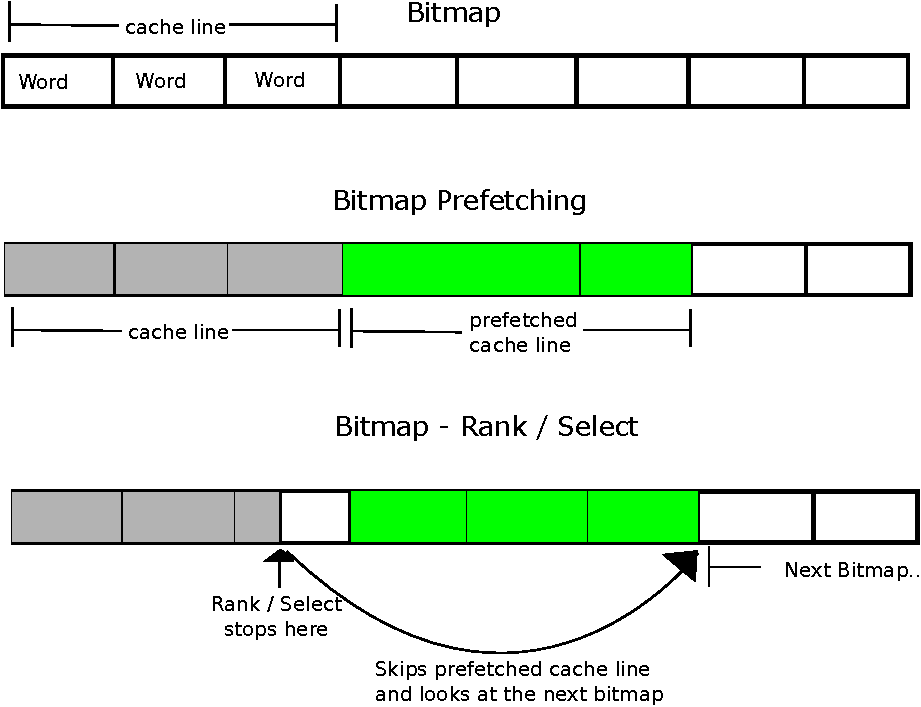
\includegraphics[width=\textwidth]{QueryPrefetchFigure.pdf}
\figureEnd



\subsection{Experiments}

\subsubsection{Queries when skewing the Wavelet Tree using uncontrolled and controlled memory layout}
In this experiment we want to test whether querying our controlled memory version of the Wavelet Tree is faster than querying the uncontrolled memory version for increasingly skewed trees. 

\paragraph{Test Setup}~\\
The general setup is as described in Section~\ref{sec:ExpNotesGeneralSetup}.
The query parameters were chosen as described in Section~\ref{sec:choiceOfQueryParameters}.
The results can be seen in Figure ~\ref{fig:NaiveRankSkewRunningTime} and \ref{fig:NaiveSelectSkewRunningTime}.

We skew the Wavelet Tree (see section~\ref{sec:SkewingTheTree}) because we believe it has better performance than not skewing it since data can then be stored sequentially in memory and reduce cache-misses because of prefetching and should then be faster to access when querying.
Skewing should also reduce branch mispredictions since branching to the right become more probable than branching to the left. 

If we look at figure ~\ref{fig:NaiveRankSkewRunningTime} and \ref{fig:NaiveSelectSkewRunningTime} we can see that the query time increases linearly with increasing skew for both controlled and uncontrolled memory layout. We also observe that the two memory layout approaches are almost equal for both rank and select queries in terms of running time.

This means we can conclude that skewing the tree is not an improvement on performance.

\paragraph{Measurements}~\\
To understand why skewing the tree is no improvement we need to figure out what causes the increase in query time. 
First we look at branch mispredictions to see if they actually decrease when we increase the skew factor.%

 
Figure~\ref{fig:NaiveVsControlledNodeMemorySkewRankQueryBMrate} and \ref{fig:NaiveVsControlledNodeMemorySkewSelectQueryBMrate} shows the branch misprediction rate for rank and select queries on a wavelet tree with increasing skew factor for both the controlled and uncontrolled memory approach. 
The branch misprediction rate is calculated by dividing the number of branch mispredictions with the total number of conditional branches.

We observe that the branch misprediction rate is decreasing as we expected. 
This means that it is not branch mispredictions that causes the increase in query time. 

We now look at cache misses to see if they can explain the increase in query time. 
The values are shown in Figure~\ref{fig:L1NaiveControlledNodeMemoryRankSkewCacheMisses} and \ref{fig:L2L3NaiveControlledNodeMemoryRankSkewCacheMisses} for Rank and in Figure~\ref{fig:L1NaiveControlledNodeMemorySelectSkewCacheMisses} and \ref{fig:L2L3NaiveControlledNodeMemorySelectSkewCacheMisses} for Select.
The same tendency as in Figure~\ref{fig:NaiveRankSkewRunningTime} and \ref{fig:NaiveSelectSkewRunningTime} is observed: 
The cache misses increase linearly with the skew factor.

The cache misses for level 1 for Naive and Controlled Memory are almost exactly equal which might be because even the smallest bitmaps fills out the cache line resulting in cache misses even when those bitmaps are accessed. 
The cache misses of level 2 and 3 for Naive and Controlled Memory are also equal. 
Based on this we can conclude that controlling the memory ourselves has no advantage over not doing so with regards to the performance of queries.

Looking at the level 2 cache miss rates for rank and select, as plotted in Figure~\ref{fig:NaiveVsControlledNodeMemorySkewRankQuery_L2_DCMrate} and \ref{fig:NaiveVsControlledNodeMemorySkewSelectQuery_L2_DCMrate} we can see that the Data Cache Miss Rate for the level 2 cache increases for higher values of skew, meaning that it is not only a matter of an increased amount of cycles caused by the higher amount of cache misses, but that more cache accesses miss as skew increase meaning that the percentage of cache misses are increasing.

Figure~\ref{fig:NaiveVsControlledNodeMemorySkewRankQueryTLB} and \ref{fig:NaiveVsControlledNodeMemorySkewSelectQueryTLB} shows TLB misses for \textproc{Rank} and \textproc{Select}. 
The TLB misses varies a lot for increasing skew and does not seem to follow any discernible pattern which makes it difficult to say anything conclusive about these graphs. 
Figure~\ref{fig:NaiveVsControlledNodeMemorySkewSelectQueryTLB} does have two peaks at skew 2.8 and 4.2 that looks somewhat alike, but we have not been able to find any good explanation as to why they occur and they do not seem to have any visible effect on the query time when looking at figure~\ref{fig:NaiveRankSkewRunningTime} and \ref{fig:NaiveSelectSkewRunningTime}.
There are no peaks in query time when skew is 2.8 or 4.2.

In the end we can conclude that skewing the tree is not an improvement. 
Controlling the memory layout of the nodes does not improve query time because all the work is being done in the bitmaps of the nodes.
It is when accessing these bitmaps that the cache misses occur.
When the tree is skewed it's hight is increased and as a result more bitmaps needs to be accessed before a query is finished. 
This produces more cache misses than when the tree is binary balanced.


\newgeometry{left=2cm,right=2cm, top=2cm, bottom=3cm}

\begin{figure}\tiny
\begin{subfigure}{0.48\textwidth}
	% GNUPLOT: LaTeX picture with Postscript
\begingroup
  \makeatletter
  \providecommand\color[2][]{%
    \GenericError{(gnuplot) \space\space\space\@spaces}{%
      Package color not loaded in conjunction with
      terminal option `colourtext'%
    }{See the gnuplot documentation for explanation.%
    }{Either use 'blacktext' in gnuplot or load the package
      color.sty in LaTeX.}%
    \renewcommand\color[2][]{}%
  }%
  \providecommand\includegraphics[2][]{%
    \GenericError{(gnuplot) \space\space\space\@spaces}{%
      Package graphicx or graphics not loaded%
    }{See the gnuplot documentation for explanation.%
    }{The gnuplot epslatex terminal needs graphicx.sty or graphics.sty.}%
    \renewcommand\includegraphics[2][]{}%
  }%
  \providecommand\rotatebox[2]{#2}%
  \@ifundefined{ifGPcolor}{%
    \newif\ifGPcolor
    \GPcolortrue
  }{}%
  \@ifundefined{ifGPblacktext}{%
    \newif\ifGPblacktext
    \GPblacktexttrue
  }{}%
  % define a \g@addto@macro without @ in the name:
  \let\gplgaddtomacro\g@addto@macro
  % define empty templates for all commands taking text:
  \gdef\gplbacktext{}%
  \gdef\gplfronttext{}%
  \makeatother
  \ifGPblacktext
    % no textcolor at all
    \def\colorrgb#1{}%
    \def\colorgray#1{}%
  \else
    % gray or color?
    \ifGPcolor
      \def\colorrgb#1{\color[rgb]{#1}}%
      \def\colorgray#1{\color[gray]{#1}}%
      \expandafter\def\csname LTw\endcsname{\color{white}}%
      \expandafter\def\csname LTb\endcsname{\color{black}}%
      \expandafter\def\csname LTa\endcsname{\color{black}}%
      \expandafter\def\csname LT0\endcsname{\color[rgb]{1,0,0}}%
      \expandafter\def\csname LT1\endcsname{\color[rgb]{0,1,0}}%
      \expandafter\def\csname LT2\endcsname{\color[rgb]{0,0,1}}%
      \expandafter\def\csname LT3\endcsname{\color[rgb]{1,0,1}}%
      \expandafter\def\csname LT4\endcsname{\color[rgb]{0,1,1}}%
      \expandafter\def\csname LT5\endcsname{\color[rgb]{1,1,0}}%
      \expandafter\def\csname LT6\endcsname{\color[rgb]{0,0,0}}%
      \expandafter\def\csname LT7\endcsname{\color[rgb]{1,0.3,0}}%
      \expandafter\def\csname LT8\endcsname{\color[rgb]{0.5,0.5,0.5}}%
    \else
      % gray
      \def\colorrgb#1{\color{black}}%
      \def\colorgray#1{\color[gray]{#1}}%
      \expandafter\def\csname LTw\endcsname{\color{white}}%
      \expandafter\def\csname LTb\endcsname{\color{black}}%
      \expandafter\def\csname LTa\endcsname{\color{black}}%
      \expandafter\def\csname LT0\endcsname{\color{black}}%
      \expandafter\def\csname LT1\endcsname{\color{black}}%
      \expandafter\def\csname LT2\endcsname{\color{black}}%
      \expandafter\def\csname LT3\endcsname{\color{black}}%
      \expandafter\def\csname LT4\endcsname{\color{black}}%
      \expandafter\def\csname LT5\endcsname{\color{black}}%
      \expandafter\def\csname LT6\endcsname{\color{black}}%
      \expandafter\def\csname LT7\endcsname{\color{black}}%
      \expandafter\def\csname LT8\endcsname{\color{black}}%
    \fi
  \fi
  \setlength{\unitlength}{0.0500bp}%
  \begin{picture}(4608.00,3600.00)%
    \gplgaddtomacro\gplbacktext{%
      \csname LTb\endcsname%
      \put(516,384){\makebox(0,0)[r]{\strut{} 0}}%
      \put(516,998){\makebox(0,0)[r]{\strut{} 0.5}}%
      \put(516,1612){\makebox(0,0)[r]{\strut{} 1}}%
      \put(516,2227){\makebox(0,0)[r]{\strut{} 1.5}}%
      \put(516,2841){\makebox(0,0)[r]{\strut{} 2}}%
      \put(516,3455){\makebox(0,0)[r]{\strut{} 2.5}}%
      \put(588,264){\makebox(0,0){\strut{} 2}}%
      \put(1063,264){\makebox(0,0){\strut{} 2.5}}%
      \put(1539,264){\makebox(0,0){\strut{} 3}}%
      \put(2014,264){\makebox(0,0){\strut{} 3.5}}%
      \put(2490,264){\makebox(0,0){\strut{} 4}}%
      \put(2965,264){\makebox(0,0){\strut{} 4.5}}%
      \put(3440,264){\makebox(0,0){\strut{} 5}}%
      \put(3916,264){\makebox(0,0){\strut{} 5.5}}%
      \put(4391,264){\makebox(0,0){\strut{} 6}}%
      \put(96,1919){\rotatebox{-270}{\makebox(0,0){\strut{}Wall Time (sec)}}}%
      \put(2489,84){\makebox(0,0){\strut{}Skew}}%
    }%
    \gplgaddtomacro\gplfronttext{%
      \csname LTb\endcsname%
      \put(1812,3332){\makebox(0,0)[r]{\strut{}NaiveInteger}}%
      \csname LTb\endcsname%
      \put(3459,3332){\makebox(0,0)[r]{\strut{}ControlledMemory}}%
    }%
    \gplbacktext
    \put(0,0){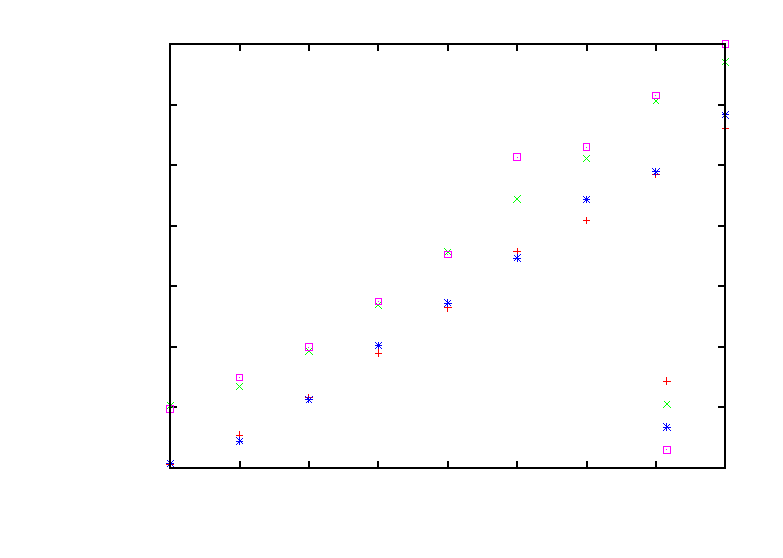
\includegraphics{naiveRankSkewRunningTime}}%
    \gplfronttext
  \end{picture}%
\endgroup

	\caption{Wall Time}
	\label{fig:NaiveRankSkewRunningTime}
\end{subfigure}
\hfill
\begin{subfigure}{0.48\textwidth}
	% GNUPLOT: LaTeX picture with Postscript
\begingroup
  \makeatletter
  \providecommand\color[2][]{%
    \GenericError{(gnuplot) \space\space\space\@spaces}{%
      Package color not loaded in conjunction with
      terminal option `colourtext'%
    }{See the gnuplot documentation for explanation.%
    }{Either use 'blacktext' in gnuplot or load the package
      color.sty in LaTeX.}%
    \renewcommand\color[2][]{}%
  }%
  \providecommand\includegraphics[2][]{%
    \GenericError{(gnuplot) \space\space\space\@spaces}{%
      Package graphicx or graphics not loaded%
    }{See the gnuplot documentation for explanation.%
    }{The gnuplot epslatex terminal needs graphicx.sty or graphics.sty.}%
    \renewcommand\includegraphics[2][]{}%
  }%
  \providecommand\rotatebox[2]{#2}%
  \@ifundefined{ifGPcolor}{%
    \newif\ifGPcolor
    \GPcolortrue
  }{}%
  \@ifundefined{ifGPblacktext}{%
    \newif\ifGPblacktext
    \GPblacktexttrue
  }{}%
  % define a \g@addto@macro without @ in the name:
  \let\gplgaddtomacro\g@addto@macro
  % define empty templates for all commands taking text:
  \gdef\gplbacktext{}%
  \gdef\gplfronttext{}%
  \makeatother
  \ifGPblacktext
    % no textcolor at all
    \def\colorrgb#1{}%
    \def\colorgray#1{}%
  \else
    % gray or color?
    \ifGPcolor
      \def\colorrgb#1{\color[rgb]{#1}}%
      \def\colorgray#1{\color[gray]{#1}}%
      \expandafter\def\csname LTw\endcsname{\color{white}}%
      \expandafter\def\csname LTb\endcsname{\color{black}}%
      \expandafter\def\csname LTa\endcsname{\color{black}}%
      \expandafter\def\csname LT0\endcsname{\color[rgb]{1,0,0}}%
      \expandafter\def\csname LT1\endcsname{\color[rgb]{0,1,0}}%
      \expandafter\def\csname LT2\endcsname{\color[rgb]{0,0,1}}%
      \expandafter\def\csname LT3\endcsname{\color[rgb]{1,0,1}}%
      \expandafter\def\csname LT4\endcsname{\color[rgb]{0,1,1}}%
      \expandafter\def\csname LT5\endcsname{\color[rgb]{1,1,0}}%
      \expandafter\def\csname LT6\endcsname{\color[rgb]{0,0,0}}%
      \expandafter\def\csname LT7\endcsname{\color[rgb]{1,0.3,0}}%
      \expandafter\def\csname LT8\endcsname{\color[rgb]{0.5,0.5,0.5}}%
    \else
      % gray
      \def\colorrgb#1{\color{black}}%
      \def\colorgray#1{\color[gray]{#1}}%
      \expandafter\def\csname LTw\endcsname{\color{white}}%
      \expandafter\def\csname LTb\endcsname{\color{black}}%
      \expandafter\def\csname LTa\endcsname{\color{black}}%
      \expandafter\def\csname LT0\endcsname{\color{black}}%
      \expandafter\def\csname LT1\endcsname{\color{black}}%
      \expandafter\def\csname LT2\endcsname{\color{black}}%
      \expandafter\def\csname LT3\endcsname{\color{black}}%
      \expandafter\def\csname LT4\endcsname{\color{black}}%
      \expandafter\def\csname LT5\endcsname{\color{black}}%
      \expandafter\def\csname LT6\endcsname{\color{black}}%
      \expandafter\def\csname LT7\endcsname{\color{black}}%
      \expandafter\def\csname LT8\endcsname{\color{black}}%
    \fi
  \fi
  \setlength{\unitlength}{0.0500bp}%
  \begin{picture}(4608.00,3600.00)%
    \gplgaddtomacro\gplbacktext{%
      \csname LTb\endcsname%
      \put(804,384){\makebox(0,0)[r]{\strut{} 0}}%
      \put(804,725){\makebox(0,0)[r]{\strut{} 2e-06}}%
      \put(804,1066){\makebox(0,0)[r]{\strut{} 4e-06}}%
      \put(804,1408){\makebox(0,0)[r]{\strut{} 6e-06}}%
      \put(804,1749){\makebox(0,0)[r]{\strut{} 8e-06}}%
      \put(804,2090){\makebox(0,0)[r]{\strut{} 1e-05}}%
      \put(804,2431){\makebox(0,0)[r]{\strut{} 1.2e-05}}%
      \put(804,2773){\makebox(0,0)[r]{\strut{} 1.4e-05}}%
      \put(804,3114){\makebox(0,0)[r]{\strut{} 1.6e-05}}%
      \put(804,3455){\makebox(0,0)[r]{\strut{} 1.8e-05}}%
      \put(876,264){\makebox(0,0){\strut{} 2}}%
      \put(1315,264){\makebox(0,0){\strut{} 2.5}}%
      \put(1755,264){\makebox(0,0){\strut{} 3}}%
      \put(2194,264){\makebox(0,0){\strut{} 3.5}}%
      \put(2634,264){\makebox(0,0){\strut{} 4}}%
      \put(3073,264){\makebox(0,0){\strut{} 4.5}}%
      \put(3512,264){\makebox(0,0){\strut{} 5}}%
      \put(3952,264){\makebox(0,0){\strut{} 5.5}}%
      \put(4391,264){\makebox(0,0){\strut{} 6}}%
      \put(96,1919){\rotatebox{-270}{\makebox(0,0){\strut{}Branch Misprediction Rate}}}%
      \put(2633,84){\makebox(0,0){\strut{}Skew}}%
    }%
    \gplgaddtomacro\gplfronttext{%
      \csname LTb\endcsname%
      \put(1889,3332){\makebox(0,0)[r]{\strut{}Naive}}%
      \csname LTb\endcsname%
      \put(3824,3332){\makebox(0,0)[r]{\strut{}ControlledNodeMemory}}%
    }%
    \gplbacktext
    \put(0,0){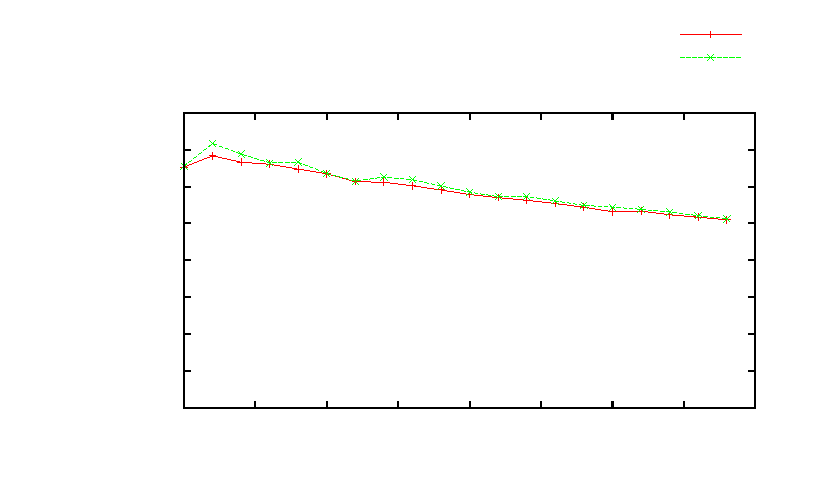
\includegraphics{NaiveVsControlledNodeMemorySkewRankQuery_BMrate}}%
    \gplfronttext
  \end{picture}%
\endgroup

	\caption{Branch Misprediction Rate}
	\label{fig:NaiveVsControlledNodeMemorySkewRankQueryBMrate}
\end{subfigure}


\begin{subfigure}{0.48\textwidth}
	% GNUPLOT: LaTeX picture with Postscript
\begingroup
  \makeatletter
  \providecommand\color[2][]{%
    \GenericError{(gnuplot) \space\space\space\@spaces}{%
      Package color not loaded in conjunction with
      terminal option `colourtext'%
    }{See the gnuplot documentation for explanation.%
    }{Either use 'blacktext' in gnuplot or load the package
      color.sty in LaTeX.}%
    \renewcommand\color[2][]{}%
  }%
  \providecommand\includegraphics[2][]{%
    \GenericError{(gnuplot) \space\space\space\@spaces}{%
      Package graphicx or graphics not loaded%
    }{See the gnuplot documentation for explanation.%
    }{The gnuplot epslatex terminal needs graphicx.sty or graphics.sty.}%
    \renewcommand\includegraphics[2][]{}%
  }%
  \providecommand\rotatebox[2]{#2}%
  \@ifundefined{ifGPcolor}{%
    \newif\ifGPcolor
    \GPcolortrue
  }{}%
  \@ifundefined{ifGPblacktext}{%
    \newif\ifGPblacktext
    \GPblacktexttrue
  }{}%
  % define a \g@addto@macro without @ in the name:
  \let\gplgaddtomacro\g@addto@macro
  % define empty templates for all commands taking text:
  \gdef\gplbacktext{}%
  \gdef\gplfronttext{}%
  \makeatother
  \ifGPblacktext
    % no textcolor at all
    \def\colorrgb#1{}%
    \def\colorgray#1{}%
  \else
    % gray or color?
    \ifGPcolor
      \def\colorrgb#1{\color[rgb]{#1}}%
      \def\colorgray#1{\color[gray]{#1}}%
      \expandafter\def\csname LTw\endcsname{\color{white}}%
      \expandafter\def\csname LTb\endcsname{\color{black}}%
      \expandafter\def\csname LTa\endcsname{\color{black}}%
      \expandafter\def\csname LT0\endcsname{\color[rgb]{1,0,0}}%
      \expandafter\def\csname LT1\endcsname{\color[rgb]{0,1,0}}%
      \expandafter\def\csname LT2\endcsname{\color[rgb]{0,0,1}}%
      \expandafter\def\csname LT3\endcsname{\color[rgb]{1,0,1}}%
      \expandafter\def\csname LT4\endcsname{\color[rgb]{0,1,1}}%
      \expandafter\def\csname LT5\endcsname{\color[rgb]{1,1,0}}%
      \expandafter\def\csname LT6\endcsname{\color[rgb]{0,0,0}}%
      \expandafter\def\csname LT7\endcsname{\color[rgb]{1,0.3,0}}%
      \expandafter\def\csname LT8\endcsname{\color[rgb]{0.5,0.5,0.5}}%
    \else
      % gray
      \def\colorrgb#1{\color{black}}%
      \def\colorgray#1{\color[gray]{#1}}%
      \expandafter\def\csname LTw\endcsname{\color{white}}%
      \expandafter\def\csname LTb\endcsname{\color{black}}%
      \expandafter\def\csname LTa\endcsname{\color{black}}%
      \expandafter\def\csname LT0\endcsname{\color{black}}%
      \expandafter\def\csname LT1\endcsname{\color{black}}%
      \expandafter\def\csname LT2\endcsname{\color{black}}%
      \expandafter\def\csname LT3\endcsname{\color{black}}%
      \expandafter\def\csname LT4\endcsname{\color{black}}%
      \expandafter\def\csname LT5\endcsname{\color{black}}%
      \expandafter\def\csname LT6\endcsname{\color{black}}%
      \expandafter\def\csname LT7\endcsname{\color{black}}%
      \expandafter\def\csname LT8\endcsname{\color{black}}%
    \fi
  \fi
  \setlength{\unitlength}{0.0500bp}%
  \begin{picture}(7488.00,4752.00)%
    \gplgaddtomacro\gplbacktext{%
      \csname LTb\endcsname%
      \put(1474,704){\makebox(0,0)[r]{\strut{} 0}}%
      \put(1474,1150){\makebox(0,0)[r]{\strut{} 5e+06}}%
      \put(1474,1596){\makebox(0,0)[r]{\strut{} 1e+07}}%
      \put(1474,2042){\makebox(0,0)[r]{\strut{} 1.5e+07}}%
      \put(1474,2489){\makebox(0,0)[r]{\strut{} 2e+07}}%
      \put(1474,2935){\makebox(0,0)[r]{\strut{} 2.5e+07}}%
      \put(1474,3381){\makebox(0,0)[r]{\strut{} 3e+07}}%
      \put(1474,3827){\makebox(0,0)[r]{\strut{} 3.5e+07}}%
      \put(1606,484){\makebox(0,0){\strut{} 2}}%
      \put(2292,484){\makebox(0,0){\strut{} 2.5}}%
      \put(2977,484){\makebox(0,0){\strut{} 3}}%
      \put(3663,484){\makebox(0,0){\strut{} 3.5}}%
      \put(4349,484){\makebox(0,0){\strut{} 4}}%
      \put(5034,484){\makebox(0,0){\strut{} 4.5}}%
      \put(5720,484){\makebox(0,0){\strut{} 5}}%
      \put(6405,484){\makebox(0,0){\strut{} 5.5}}%
      \put(7091,484){\makebox(0,0){\strut{} 6}}%
      \put(176,2265){\rotatebox{-270}{\makebox(0,0){\strut{}Cache Misses}}}%
      \put(4348,154){\makebox(0,0){\strut{}Skew}}%
    }%
    \gplgaddtomacro\gplfronttext{%
      \csname LTb\endcsname%
      \put(6236,4579){\makebox(0,0)[r]{\strut{}Naive L1 $mr\hat{\sigma}=$0.041 $avg\hat{\sigma}=$0.02}}%
      \csname LTb\endcsname%
      \put(6236,4359){\makebox(0,0)[r]{\strut{}ControlledNodeMemory L1 $mr\hat{\sigma}=$0.046 $avg\hat{\sigma}=$0.02}}%
    }%
    \gplbacktext
    \put(0,0){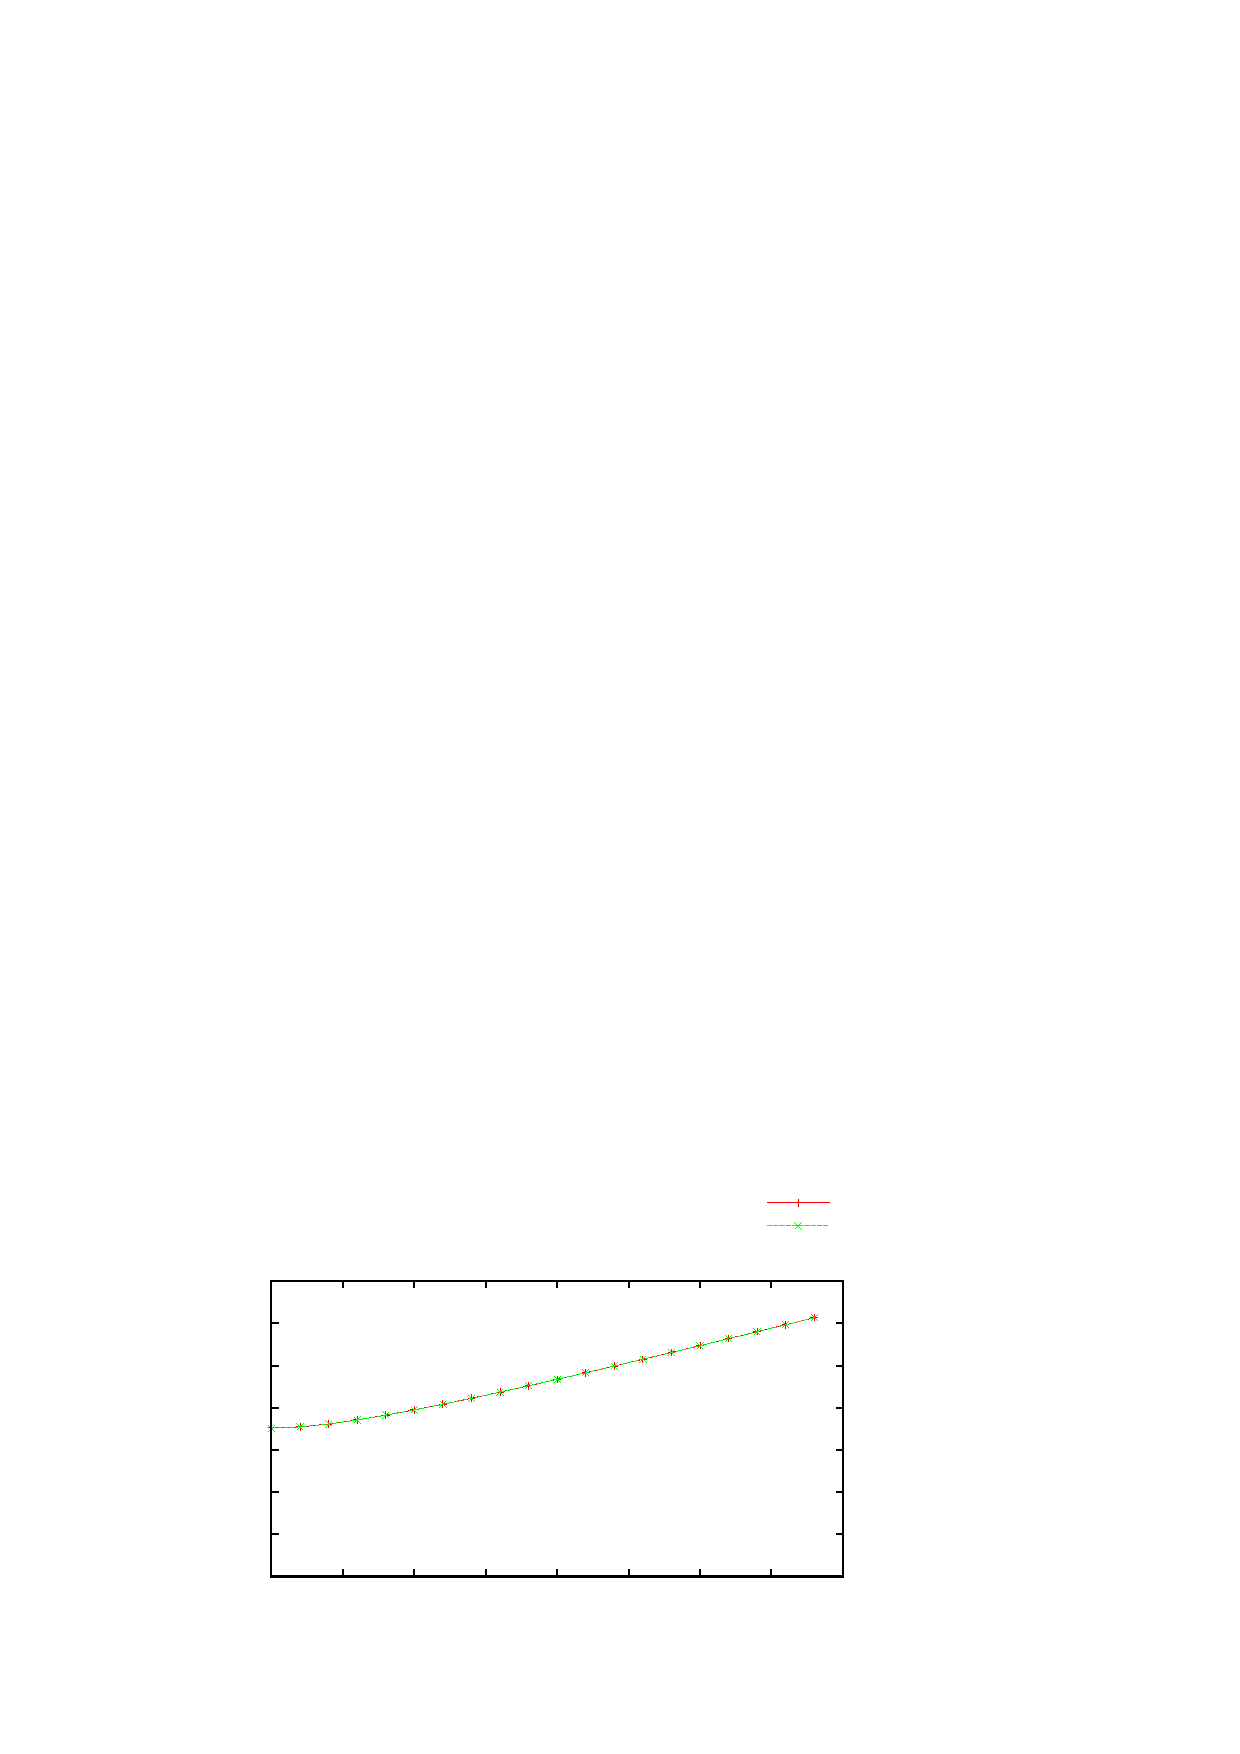
\includegraphics{L1NaiveVsControlledNodeMemorySkewRankQueryCacheMisses}}%
    \gplfronttext
  \end{picture}%
\endgroup

	\caption{Level 1 Data Cache Misses}
	\label{fig:L1NaiveControlledNodeMemoryRankSkewCacheMisses}
\end{subfigure}
\hfill
\begin{subfigure}{0.48\textwidth}
 	% GNUPLOT: LaTeX picture with Postscript
\begingroup
  \makeatletter
  \providecommand\color[2][]{%
    \GenericError{(gnuplot) \space\space\space\@spaces}{%
      Package color not loaded in conjunction with
      terminal option `colourtext'%
    }{See the gnuplot documentation for explanation.%
    }{Either use 'blacktext' in gnuplot or load the package
      color.sty in LaTeX.}%
    \renewcommand\color[2][]{}%
  }%
  \providecommand\includegraphics[2][]{%
    \GenericError{(gnuplot) \space\space\space\@spaces}{%
      Package graphicx or graphics not loaded%
    }{See the gnuplot documentation for explanation.%
    }{The gnuplot epslatex terminal needs graphicx.sty or graphics.sty.}%
    \renewcommand\includegraphics[2][]{}%
  }%
  \providecommand\rotatebox[2]{#2}%
  \@ifundefined{ifGPcolor}{%
    \newif\ifGPcolor
    \GPcolortrue
  }{}%
  \@ifundefined{ifGPblacktext}{%
    \newif\ifGPblacktext
    \GPblacktexttrue
  }{}%
  % define a \g@addto@macro without @ in the name:
  \let\gplgaddtomacro\g@addto@macro
  % define empty templates for all commands taking text:
  \gdef\gplbacktext{}%
  \gdef\gplfronttext{}%
  \makeatother
  \ifGPblacktext
    % no textcolor at all
    \def\colorrgb#1{}%
    \def\colorgray#1{}%
  \else
    % gray or color?
    \ifGPcolor
      \def\colorrgb#1{\color[rgb]{#1}}%
      \def\colorgray#1{\color[gray]{#1}}%
      \expandafter\def\csname LTw\endcsname{\color{white}}%
      \expandafter\def\csname LTb\endcsname{\color{black}}%
      \expandafter\def\csname LTa\endcsname{\color{black}}%
      \expandafter\def\csname LT0\endcsname{\color[rgb]{1,0,0}}%
      \expandafter\def\csname LT1\endcsname{\color[rgb]{0,1,0}}%
      \expandafter\def\csname LT2\endcsname{\color[rgb]{0,0,1}}%
      \expandafter\def\csname LT3\endcsname{\color[rgb]{1,0,1}}%
      \expandafter\def\csname LT4\endcsname{\color[rgb]{0,1,1}}%
      \expandafter\def\csname LT5\endcsname{\color[rgb]{1,1,0}}%
      \expandafter\def\csname LT6\endcsname{\color[rgb]{0,0,0}}%
      \expandafter\def\csname LT7\endcsname{\color[rgb]{1,0.3,0}}%
      \expandafter\def\csname LT8\endcsname{\color[rgb]{0.5,0.5,0.5}}%
    \else
      % gray
      \def\colorrgb#1{\color{black}}%
      \def\colorgray#1{\color[gray]{#1}}%
      \expandafter\def\csname LTw\endcsname{\color{white}}%
      \expandafter\def\csname LTb\endcsname{\color{black}}%
      \expandafter\def\csname LTa\endcsname{\color{black}}%
      \expandafter\def\csname LT0\endcsname{\color{black}}%
      \expandafter\def\csname LT1\endcsname{\color{black}}%
      \expandafter\def\csname LT2\endcsname{\color{black}}%
      \expandafter\def\csname LT3\endcsname{\color{black}}%
      \expandafter\def\csname LT4\endcsname{\color{black}}%
      \expandafter\def\csname LT5\endcsname{\color{black}}%
      \expandafter\def\csname LT6\endcsname{\color{black}}%
      \expandafter\def\csname LT7\endcsname{\color{black}}%
      \expandafter\def\csname LT8\endcsname{\color{black}}%
    \fi
  \fi
  \setlength{\unitlength}{0.0500bp}%
  \begin{picture}(8062.00,4752.00)%
    \gplgaddtomacro\gplbacktext{%
      \csname LTb\endcsname%
      \put(1474,704){\makebox(0,0)[r]{\strut{} 0}}%
      \put(1474,1461){\makebox(0,0)[r]{\strut{} 500000}}%
      \put(1474,2217){\makebox(0,0)[r]{\strut{} 1e+06}}%
      \put(1474,2974){\makebox(0,0)[r]{\strut{} 1.5e+06}}%
      \put(1474,3730){\makebox(0,0)[r]{\strut{} 2e+06}}%
      \put(1474,4487){\makebox(0,0)[r]{\strut{} 2.5e+06}}%
      \put(1606,484){\makebox(0,0){\strut{} 2}}%
      \put(2363,484){\makebox(0,0){\strut{} 2.5}}%
      \put(3121,484){\makebox(0,0){\strut{} 3}}%
      \put(3878,484){\makebox(0,0){\strut{} 3.5}}%
      \put(4636,484){\makebox(0,0){\strut{} 4}}%
      \put(5393,484){\makebox(0,0){\strut{} 4.5}}%
      \put(6150,484){\makebox(0,0){\strut{} 5}}%
      \put(6908,484){\makebox(0,0){\strut{} 5.5}}%
      \put(7665,484){\makebox(0,0){\strut{} 6}}%
      \put(176,2595){\rotatebox{-270}{\makebox(0,0){\strut{}Cache Misses}}}%
      \put(4635,154){\makebox(0,0){\strut{}Skew}}%
    }%
    \gplgaddtomacro\gplfronttext{%
      \csname LTb\endcsname%
      \put(6226,4314){\makebox(0,0)[r]{\strut{}Naive L2 $mr\sigma=$14.203}}%
      \csname LTb\endcsname%
      \put(6226,4094){\makebox(0,0)[r]{\strut{}Naive L3 $mr\sigma=$26.648}}%
      \csname LTb\endcsname%
      \put(6226,3874){\makebox(0,0)[r]{\strut{}ControlledNodeMemory L2 $mr\sigma=$52.05}}%
      \csname LTb\endcsname%
      \put(6226,3654){\makebox(0,0)[r]{\strut{}ControlledNodeMemory L3 $mr\sigma=$62.695}}%
    }%
    \gplbacktext
    \put(0,0){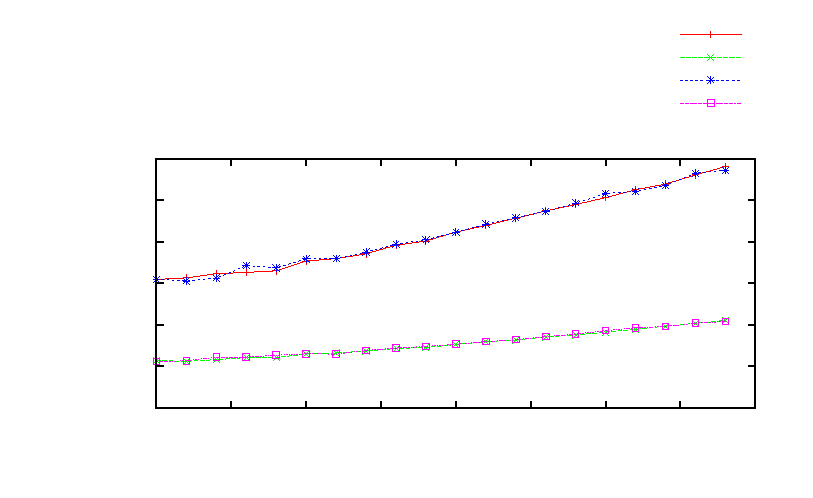
\includegraphics{L2L3NaiveVsControlledNodeMemorySkewRankQueryCacheMisses}}%
    \gplfronttext
  \end{picture}%
\endgroup

	\caption{Level 2 Data and 3 Total Cache Misses}
	\label{fig:L2L3NaiveControlledNodeMemoryRankSkewCacheMisses}
\end{subfigure}

\begin{subfigure}{0.48\textwidth}
	% GNUPLOT: LaTeX picture with Postscript
\begingroup
  \makeatletter
  \providecommand\color[2][]{%
    \GenericError{(gnuplot) \space\space\space\@spaces}{%
      Package color not loaded in conjunction with
      terminal option `colourtext'%
    }{See the gnuplot documentation for explanation.%
    }{Either use 'blacktext' in gnuplot or load the package
      color.sty in LaTeX.}%
    \renewcommand\color[2][]{}%
  }%
  \providecommand\includegraphics[2][]{%
    \GenericError{(gnuplot) \space\space\space\@spaces}{%
      Package graphicx or graphics not loaded%
    }{See the gnuplot documentation for explanation.%
    }{The gnuplot epslatex terminal needs graphicx.sty or graphics.sty.}%
    \renewcommand\includegraphics[2][]{}%
  }%
  \providecommand\rotatebox[2]{#2}%
  \@ifundefined{ifGPcolor}{%
    \newif\ifGPcolor
    \GPcolortrue
  }{}%
  \@ifundefined{ifGPblacktext}{%
    \newif\ifGPblacktext
    \GPblacktexttrue
  }{}%
  % define a \g@addto@macro without @ in the name:
  \let\gplgaddtomacro\g@addto@macro
  % define empty templates for all commands taking text:
  \gdef\gplbacktext{}%
  \gdef\gplfronttext{}%
  \makeatother
  \ifGPblacktext
    % no textcolor at all
    \def\colorrgb#1{}%
    \def\colorgray#1{}%
  \else
    % gray or color?
    \ifGPcolor
      \def\colorrgb#1{\color[rgb]{#1}}%
      \def\colorgray#1{\color[gray]{#1}}%
      \expandafter\def\csname LTw\endcsname{\color{white}}%
      \expandafter\def\csname LTb\endcsname{\color{black}}%
      \expandafter\def\csname LTa\endcsname{\color{black}}%
      \expandafter\def\csname LT0\endcsname{\color[rgb]{1,0,0}}%
      \expandafter\def\csname LT1\endcsname{\color[rgb]{0,1,0}}%
      \expandafter\def\csname LT2\endcsname{\color[rgb]{0,0,1}}%
      \expandafter\def\csname LT3\endcsname{\color[rgb]{1,0,1}}%
      \expandafter\def\csname LT4\endcsname{\color[rgb]{0,1,1}}%
      \expandafter\def\csname LT5\endcsname{\color[rgb]{1,1,0}}%
      \expandafter\def\csname LT6\endcsname{\color[rgb]{0,0,0}}%
      \expandafter\def\csname LT7\endcsname{\color[rgb]{1,0.3,0}}%
      \expandafter\def\csname LT8\endcsname{\color[rgb]{0.5,0.5,0.5}}%
    \else
      % gray
      \def\colorrgb#1{\color{black}}%
      \def\colorgray#1{\color[gray]{#1}}%
      \expandafter\def\csname LTw\endcsname{\color{white}}%
      \expandafter\def\csname LTb\endcsname{\color{black}}%
      \expandafter\def\csname LTa\endcsname{\color{black}}%
      \expandafter\def\csname LT0\endcsname{\color{black}}%
      \expandafter\def\csname LT1\endcsname{\color{black}}%
      \expandafter\def\csname LT2\endcsname{\color{black}}%
      \expandafter\def\csname LT3\endcsname{\color{black}}%
      \expandafter\def\csname LT4\endcsname{\color{black}}%
      \expandafter\def\csname LT5\endcsname{\color{black}}%
      \expandafter\def\csname LT6\endcsname{\color{black}}%
      \expandafter\def\csname LT7\endcsname{\color{black}}%
      \expandafter\def\csname LT8\endcsname{\color{black}}%
    \fi
  \fi
  \setlength{\unitlength}{0.0500bp}%
  \begin{picture}(7488.00,4464.00)%
    \gplgaddtomacro\gplbacktext{%
      \csname LTb\endcsname%
      \put(1078,704){\makebox(0,0)[r]{\strut{} 0}}%
      \put(1078,1058){\makebox(0,0)[r]{\strut{} 0.01}}%
      \put(1078,1413){\makebox(0,0)[r]{\strut{} 0.02}}%
      \put(1078,1767){\makebox(0,0)[r]{\strut{} 0.03}}%
      \put(1078,2122){\makebox(0,0)[r]{\strut{} 0.04}}%
      \put(1078,2476){\makebox(0,0)[r]{\strut{} 0.05}}%
      \put(1078,2830){\makebox(0,0)[r]{\strut{} 0.06}}%
      \put(1078,3185){\makebox(0,0)[r]{\strut{} 0.07}}%
      \put(1078,3539){\makebox(0,0)[r]{\strut{} 0.08}}%
      \put(1210,484){\makebox(0,0){\strut{} 2}}%
      \put(1945,484){\makebox(0,0){\strut{} 2.5}}%
      \put(2680,484){\makebox(0,0){\strut{} 3}}%
      \put(3415,484){\makebox(0,0){\strut{} 3.5}}%
      \put(4151,484){\makebox(0,0){\strut{} 4}}%
      \put(4886,484){\makebox(0,0){\strut{} 4.5}}%
      \put(5621,484){\makebox(0,0){\strut{} 5}}%
      \put(6356,484){\makebox(0,0){\strut{} 5.5}}%
      \put(7091,484){\makebox(0,0){\strut{} 6}}%
      \put(176,2121){\rotatebox{-270}{\makebox(0,0){\strut{}L2 Cache miss rate}}}%
      \put(4150,154){\makebox(0,0){\strut{}Skew}}%
    }%
    \gplgaddtomacro\gplfronttext{%
      \csname LTb\endcsname%
      \put(6236,4291){\makebox(0,0)[r]{\strut{}Naive $mr\hat{\sigma}=$14.395 $avg\hat{\sigma}=$4.57}}%
      \csname LTb\endcsname%
      \put(6236,4071){\makebox(0,0)[r]{\strut{}ControlledNodeMemory $mr\hat{\sigma}=$55.041 $avg\hat{\sigma}=$20.23}}%
    }%
    \gplbacktext
    \put(0,0){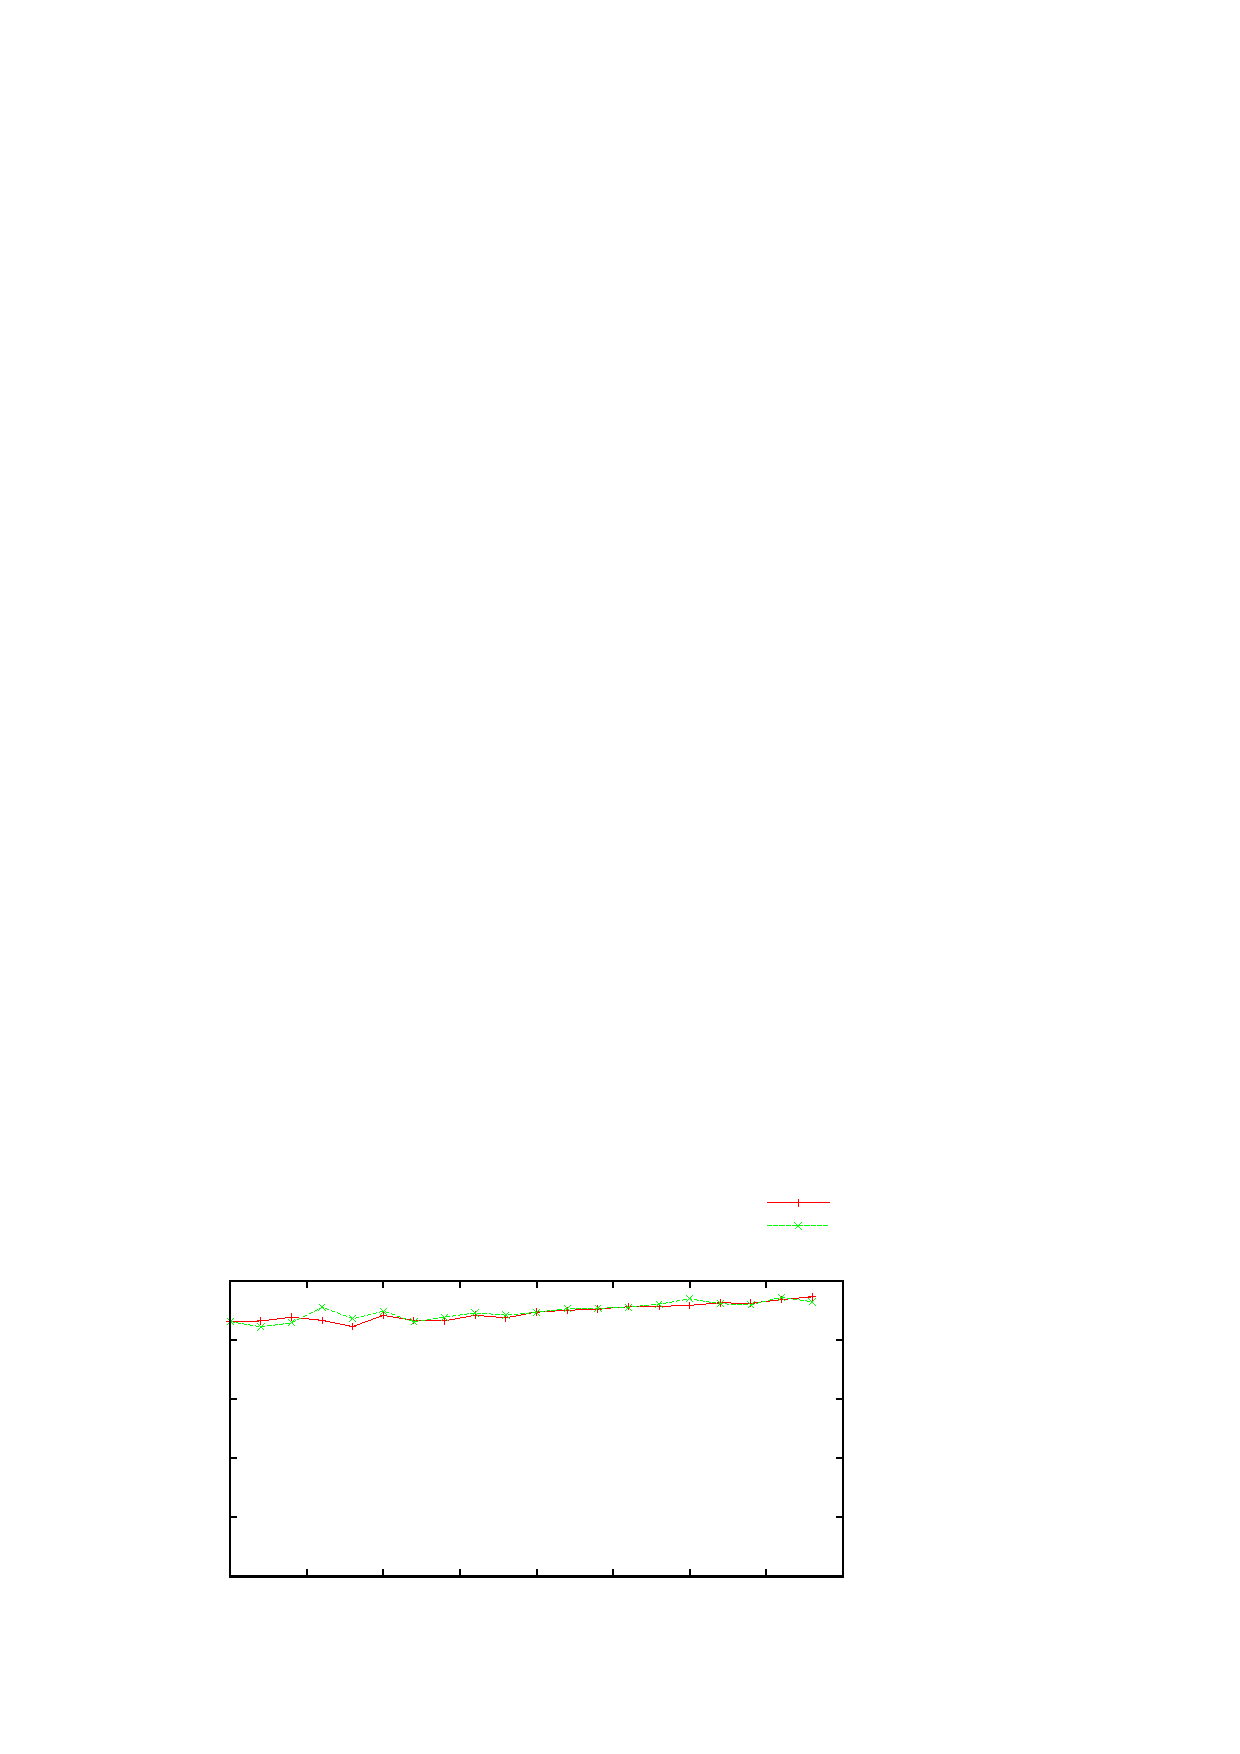
\includegraphics{NaiveVsControlledNodeMemorySkewRankQuery_L2_DCMrate}}%
    \gplfronttext
  \end{picture}%
\endgroup

	\caption{Level 2 Data Cache Miss Rate}
	\label{fig:NaiveVsControlledNodeMemorySkewRankQuery_L2_DCMrate}
\end{subfigure}
\hfill
\begin{subfigure}{0.48\textwidth}
	% GNUPLOT: LaTeX picture with Postscript
\begingroup
  \makeatletter
  \providecommand\color[2][]{%
    \GenericError{(gnuplot) \space\space\space\@spaces}{%
      Package color not loaded in conjunction with
      terminal option `colourtext'%
    }{See the gnuplot documentation for explanation.%
    }{Either use 'blacktext' in gnuplot or load the package
      color.sty in LaTeX.}%
    \renewcommand\color[2][]{}%
  }%
  \providecommand\includegraphics[2][]{%
    \GenericError{(gnuplot) \space\space\space\@spaces}{%
      Package graphicx or graphics not loaded%
    }{See the gnuplot documentation for explanation.%
    }{The gnuplot epslatex terminal needs graphicx.sty or graphics.sty.}%
    \renewcommand\includegraphics[2][]{}%
  }%
  \providecommand\rotatebox[2]{#2}%
  \@ifundefined{ifGPcolor}{%
    \newif\ifGPcolor
    \GPcolortrue
  }{}%
  \@ifundefined{ifGPblacktext}{%
    \newif\ifGPblacktext
    \GPblacktexttrue
  }{}%
  % define a \g@addto@macro without @ in the name:
  \let\gplgaddtomacro\g@addto@macro
  % define empty templates for all commands taking text:
  \gdef\gplbacktext{}%
  \gdef\gplfronttext{}%
  \makeatother
  \ifGPblacktext
    % no textcolor at all
    \def\colorrgb#1{}%
    \def\colorgray#1{}%
  \else
    % gray or color?
    \ifGPcolor
      \def\colorrgb#1{\color[rgb]{#1}}%
      \def\colorgray#1{\color[gray]{#1}}%
      \expandafter\def\csname LTw\endcsname{\color{white}}%
      \expandafter\def\csname LTb\endcsname{\color{black}}%
      \expandafter\def\csname LTa\endcsname{\color{black}}%
      \expandafter\def\csname LT0\endcsname{\color[rgb]{1,0,0}}%
      \expandafter\def\csname LT1\endcsname{\color[rgb]{0,1,0}}%
      \expandafter\def\csname LT2\endcsname{\color[rgb]{0,0,1}}%
      \expandafter\def\csname LT3\endcsname{\color[rgb]{1,0,1}}%
      \expandafter\def\csname LT4\endcsname{\color[rgb]{0,1,1}}%
      \expandafter\def\csname LT5\endcsname{\color[rgb]{1,1,0}}%
      \expandafter\def\csname LT6\endcsname{\color[rgb]{0,0,0}}%
      \expandafter\def\csname LT7\endcsname{\color[rgb]{1,0.3,0}}%
      \expandafter\def\csname LT8\endcsname{\color[rgb]{0.5,0.5,0.5}}%
    \else
      % gray
      \def\colorrgb#1{\color{black}}%
      \def\colorgray#1{\color[gray]{#1}}%
      \expandafter\def\csname LTw\endcsname{\color{white}}%
      \expandafter\def\csname LTb\endcsname{\color{black}}%
      \expandafter\def\csname LTa\endcsname{\color{black}}%
      \expandafter\def\csname LT0\endcsname{\color{black}}%
      \expandafter\def\csname LT1\endcsname{\color{black}}%
      \expandafter\def\csname LT2\endcsname{\color{black}}%
      \expandafter\def\csname LT3\endcsname{\color{black}}%
      \expandafter\def\csname LT4\endcsname{\color{black}}%
      \expandafter\def\csname LT5\endcsname{\color{black}}%
      \expandafter\def\csname LT6\endcsname{\color{black}}%
      \expandafter\def\csname LT7\endcsname{\color{black}}%
      \expandafter\def\csname LT8\endcsname{\color{black}}%
    \fi
  \fi
  \setlength{\unitlength}{0.0500bp}%
  \begin{picture}(4608.00,3600.00)%
    \gplgaddtomacro\gplbacktext{%
      \csname LTb\endcsname%
      \put(804,384){\makebox(0,0)[r]{\strut{} 0}}%
      \put(804,823){\makebox(0,0)[r]{\strut{} 200000}}%
      \put(804,1261){\makebox(0,0)[r]{\strut{} 400000}}%
      \put(804,1700){\makebox(0,0)[r]{\strut{} 600000}}%
      \put(804,2139){\makebox(0,0)[r]{\strut{} 800000}}%
      \put(804,2578){\makebox(0,0)[r]{\strut{} 1e+06}}%
      \put(804,3016){\makebox(0,0)[r]{\strut{} 1.2e+06}}%
      \put(804,3455){\makebox(0,0)[r]{\strut{} 1.4e+06}}%
      \put(876,264){\makebox(0,0){\strut{} 2}}%
      \put(1315,264){\makebox(0,0){\strut{} 2.5}}%
      \put(1755,264){\makebox(0,0){\strut{} 3}}%
      \put(2194,264){\makebox(0,0){\strut{} 3.5}}%
      \put(2634,264){\makebox(0,0){\strut{} 4}}%
      \put(3073,264){\makebox(0,0){\strut{} 4.5}}%
      \put(3512,264){\makebox(0,0){\strut{} 5}}%
      \put(3952,264){\makebox(0,0){\strut{} 5.5}}%
      \put(4391,264){\makebox(0,0){\strut{} 6}}%
      \put(96,1919){\rotatebox{-270}{\makebox(0,0){\strut{}TLB}}}%
      \put(2633,84){\makebox(0,0){\strut{}Skew}}%
    }%
    \gplgaddtomacro\gplfronttext{%
      \csname LTb\endcsname%
      \put(1889,3332){\makebox(0,0)[r]{\strut{}Naive}}%
      \csname LTb\endcsname%
      \put(3824,3332){\makebox(0,0)[r]{\strut{}ControlledNodeMemory}}%
    }%
    \gplbacktext
    \put(0,0){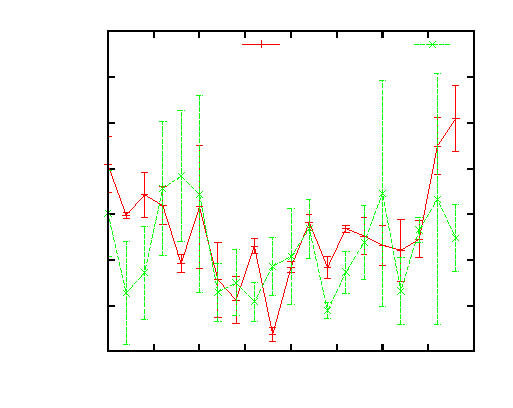
\includegraphics{NaiveVsControlledNodeMemorySkewRankQueryTLB}}%
    \gplfronttext
  \end{picture}%
\endgroup

	\caption{TLB Misses}
	\label{fig:NaiveVsControlledNodeMemorySkewRankQueryTLB}
\end{subfigure}

\caption{Various measurements for Rank queries on NaiveInteger and ControlledNodeMemory wavelet trees with various skew.}
\label{fig:NaiveVsControlledNodeMemorySkewRankQuery}

\end{figure}






\begin{figure}\tiny
\begin{subfigure}{0.48\textwidth}
	% GNUPLOT: LaTeX picture with Postscript
\begingroup
  \makeatletter
  \providecommand\color[2][]{%
    \GenericError{(gnuplot) \space\space\space\@spaces}{%
      Package color not loaded in conjunction with
      terminal option `colourtext'%
    }{See the gnuplot documentation for explanation.%
    }{Either use 'blacktext' in gnuplot or load the package
      color.sty in LaTeX.}%
    \renewcommand\color[2][]{}%
  }%
  \providecommand\includegraphics[2][]{%
    \GenericError{(gnuplot) \space\space\space\@spaces}{%
      Package graphicx or graphics not loaded%
    }{See the gnuplot documentation for explanation.%
    }{The gnuplot epslatex terminal needs graphicx.sty or graphics.sty.}%
    \renewcommand\includegraphics[2][]{}%
  }%
  \providecommand\rotatebox[2]{#2}%
  \@ifundefined{ifGPcolor}{%
    \newif\ifGPcolor
    \GPcolortrue
  }{}%
  \@ifundefined{ifGPblacktext}{%
    \newif\ifGPblacktext
    \GPblacktexttrue
  }{}%
  % define a \g@addto@macro without @ in the name:
  \let\gplgaddtomacro\g@addto@macro
  % define empty templates for all commands taking text:
  \gdef\gplbacktext{}%
  \gdef\gplfronttext{}%
  \makeatother
  \ifGPblacktext
    % no textcolor at all
    \def\colorrgb#1{}%
    \def\colorgray#1{}%
  \else
    % gray or color?
    \ifGPcolor
      \def\colorrgb#1{\color[rgb]{#1}}%
      \def\colorgray#1{\color[gray]{#1}}%
      \expandafter\def\csname LTw\endcsname{\color{white}}%
      \expandafter\def\csname LTb\endcsname{\color{black}}%
      \expandafter\def\csname LTa\endcsname{\color{black}}%
      \expandafter\def\csname LT0\endcsname{\color[rgb]{1,0,0}}%
      \expandafter\def\csname LT1\endcsname{\color[rgb]{0,1,0}}%
      \expandafter\def\csname LT2\endcsname{\color[rgb]{0,0,1}}%
      \expandafter\def\csname LT3\endcsname{\color[rgb]{1,0,1}}%
      \expandafter\def\csname LT4\endcsname{\color[rgb]{0,1,1}}%
      \expandafter\def\csname LT5\endcsname{\color[rgb]{1,1,0}}%
      \expandafter\def\csname LT6\endcsname{\color[rgb]{0,0,0}}%
      \expandafter\def\csname LT7\endcsname{\color[rgb]{1,0.3,0}}%
      \expandafter\def\csname LT8\endcsname{\color[rgb]{0.5,0.5,0.5}}%
    \else
      % gray
      \def\colorrgb#1{\color{black}}%
      \def\colorgray#1{\color[gray]{#1}}%
      \expandafter\def\csname LTw\endcsname{\color{white}}%
      \expandafter\def\csname LTb\endcsname{\color{black}}%
      \expandafter\def\csname LTa\endcsname{\color{black}}%
      \expandafter\def\csname LT0\endcsname{\color{black}}%
      \expandafter\def\csname LT1\endcsname{\color{black}}%
      \expandafter\def\csname LT2\endcsname{\color{black}}%
      \expandafter\def\csname LT3\endcsname{\color{black}}%
      \expandafter\def\csname LT4\endcsname{\color{black}}%
      \expandafter\def\csname LT5\endcsname{\color{black}}%
      \expandafter\def\csname LT6\endcsname{\color{black}}%
      \expandafter\def\csname LT7\endcsname{\color{black}}%
      \expandafter\def\csname LT8\endcsname{\color{black}}%
    \fi
  \fi
  \setlength{\unitlength}{0.0500bp}%
  \begin{picture}(4608.00,3600.00)%
    \gplgaddtomacro\gplbacktext{%
      \csname LTb\endcsname%
      \put(516,384){\makebox(0,0)[r]{\strut{} 0}}%
      \put(516,896){\makebox(0,0)[r]{\strut{} 0.5}}%
      \put(516,1408){\makebox(0,0)[r]{\strut{} 1}}%
      \put(516,1920){\makebox(0,0)[r]{\strut{} 1.5}}%
      \put(516,2431){\makebox(0,0)[r]{\strut{} 2}}%
      \put(516,2943){\makebox(0,0)[r]{\strut{} 2.5}}%
      \put(516,3455){\makebox(0,0)[r]{\strut{} 3}}%
      \put(588,264){\makebox(0,0){\strut{} 2}}%
      \put(1063,264){\makebox(0,0){\strut{} 2.5}}%
      \put(1539,264){\makebox(0,0){\strut{} 3}}%
      \put(2014,264){\makebox(0,0){\strut{} 3.5}}%
      \put(2490,264){\makebox(0,0){\strut{} 4}}%
      \put(2965,264){\makebox(0,0){\strut{} 4.5}}%
      \put(3440,264){\makebox(0,0){\strut{} 5}}%
      \put(3916,264){\makebox(0,0){\strut{} 5.5}}%
      \put(4391,264){\makebox(0,0){\strut{} 6}}%
      \put(96,1919){\rotatebox{-270}{\makebox(0,0){\strut{}Wall Time (sec)}}}%
      \put(2489,84){\makebox(0,0){\strut{}Skew}}%
    }%
    \gplgaddtomacro\gplfronttext{%
      \csname LTb\endcsname%
      \put(1812,3332){\makebox(0,0)[r]{\strut{}NaiveInteger}}%
      \csname LTb\endcsname%
      \put(3459,3332){\makebox(0,0)[r]{\strut{}ControlledMemory}}%
    }%
    \gplbacktext
    \put(0,0){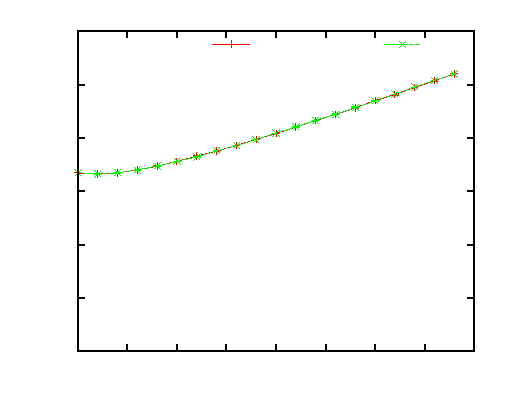
\includegraphics{naiveSelectSkewRunningTime}}%
    \gplfronttext
  \end{picture}%
\endgroup

	\caption{Wall Time}
	\label{fig:NaiveSelectSkewRunningTime}
\end{subfigure}
\hfill
\begin{subfigure}{0.48\textwidth}
	% GNUPLOT: LaTeX picture with Postscript
\begingroup
  \makeatletter
  \providecommand\color[2][]{%
    \GenericError{(gnuplot) \space\space\space\@spaces}{%
      Package color not loaded in conjunction with
      terminal option `colourtext'%
    }{See the gnuplot documentation for explanation.%
    }{Either use 'blacktext' in gnuplot or load the package
      color.sty in LaTeX.}%
    \renewcommand\color[2][]{}%
  }%
  \providecommand\includegraphics[2][]{%
    \GenericError{(gnuplot) \space\space\space\@spaces}{%
      Package graphicx or graphics not loaded%
    }{See the gnuplot documentation for explanation.%
    }{The gnuplot epslatex terminal needs graphicx.sty or graphics.sty.}%
    \renewcommand\includegraphics[2][]{}%
  }%
  \providecommand\rotatebox[2]{#2}%
  \@ifundefined{ifGPcolor}{%
    \newif\ifGPcolor
    \GPcolortrue
  }{}%
  \@ifundefined{ifGPblacktext}{%
    \newif\ifGPblacktext
    \GPblacktexttrue
  }{}%
  % define a \g@addto@macro without @ in the name:
  \let\gplgaddtomacro\g@addto@macro
  % define empty templates for all commands taking text:
  \gdef\gplbacktext{}%
  \gdef\gplfronttext{}%
  \makeatother
  \ifGPblacktext
    % no textcolor at all
    \def\colorrgb#1{}%
    \def\colorgray#1{}%
  \else
    % gray or color?
    \ifGPcolor
      \def\colorrgb#1{\color[rgb]{#1}}%
      \def\colorgray#1{\color[gray]{#1}}%
      \expandafter\def\csname LTw\endcsname{\color{white}}%
      \expandafter\def\csname LTb\endcsname{\color{black}}%
      \expandafter\def\csname LTa\endcsname{\color{black}}%
      \expandafter\def\csname LT0\endcsname{\color[rgb]{1,0,0}}%
      \expandafter\def\csname LT1\endcsname{\color[rgb]{0,1,0}}%
      \expandafter\def\csname LT2\endcsname{\color[rgb]{0,0,1}}%
      \expandafter\def\csname LT3\endcsname{\color[rgb]{1,0,1}}%
      \expandafter\def\csname LT4\endcsname{\color[rgb]{0,1,1}}%
      \expandafter\def\csname LT5\endcsname{\color[rgb]{1,1,0}}%
      \expandafter\def\csname LT6\endcsname{\color[rgb]{0,0,0}}%
      \expandafter\def\csname LT7\endcsname{\color[rgb]{1,0.3,0}}%
      \expandafter\def\csname LT8\endcsname{\color[rgb]{0.5,0.5,0.5}}%
    \else
      % gray
      \def\colorrgb#1{\color{black}}%
      \def\colorgray#1{\color[gray]{#1}}%
      \expandafter\def\csname LTw\endcsname{\color{white}}%
      \expandafter\def\csname LTb\endcsname{\color{black}}%
      \expandafter\def\csname LTa\endcsname{\color{black}}%
      \expandafter\def\csname LT0\endcsname{\color{black}}%
      \expandafter\def\csname LT1\endcsname{\color{black}}%
      \expandafter\def\csname LT2\endcsname{\color{black}}%
      \expandafter\def\csname LT3\endcsname{\color{black}}%
      \expandafter\def\csname LT4\endcsname{\color{black}}%
      \expandafter\def\csname LT5\endcsname{\color{black}}%
      \expandafter\def\csname LT6\endcsname{\color{black}}%
      \expandafter\def\csname LT7\endcsname{\color{black}}%
      \expandafter\def\csname LT8\endcsname{\color{black}}%
    \fi
  \fi
  \setlength{\unitlength}{0.0500bp}%
  \begin{picture}(7488.00,4752.00)%
    \gplgaddtomacro\gplbacktext{%
      \csname LTb\endcsname%
      \put(1210,704){\makebox(0,0)[r]{\strut{} 0}}%
      \put(1210,1329){\makebox(0,0)[r]{\strut{} 0.005}}%
      \put(1210,1953){\makebox(0,0)[r]{\strut{} 0.01}}%
      \put(1210,2578){\makebox(0,0)[r]{\strut{} 0.015}}%
      \put(1210,3202){\makebox(0,0)[r]{\strut{} 0.02}}%
      \put(1210,3827){\makebox(0,0)[r]{\strut{} 0.025}}%
      \put(1342,484){\makebox(0,0){\strut{} 2}}%
      \put(2061,484){\makebox(0,0){\strut{} 2.5}}%
      \put(2779,484){\makebox(0,0){\strut{} 3}}%
      \put(3498,484){\makebox(0,0){\strut{} 3.5}}%
      \put(4217,484){\makebox(0,0){\strut{} 4}}%
      \put(4935,484){\makebox(0,0){\strut{} 4.5}}%
      \put(5654,484){\makebox(0,0){\strut{} 5}}%
      \put(6372,484){\makebox(0,0){\strut{} 5.5}}%
      \put(7091,484){\makebox(0,0){\strut{} 6}}%
      \put(176,2265){\rotatebox{-270}{\makebox(0,0){\strut{}Branch Misprediction Rate}}}%
      \put(4216,154){\makebox(0,0){\strut{}Skew}}%
    }%
    \gplgaddtomacro\gplfronttext{%
      \csname LTb\endcsname%
      \put(6236,4579){\makebox(0,0)[r]{\strut{}Naive $mr\hat{\sigma}=$0.136 $avg\hat{\sigma}=$0.09}}%
      \csname LTb\endcsname%
      \put(6236,4359){\makebox(0,0)[r]{\strut{}ControlledNodeMemory $mr\hat{\sigma}=$0.789 $avg\hat{\sigma}=$0.17}}%
    }%
    \gplbacktext
    \put(0,0){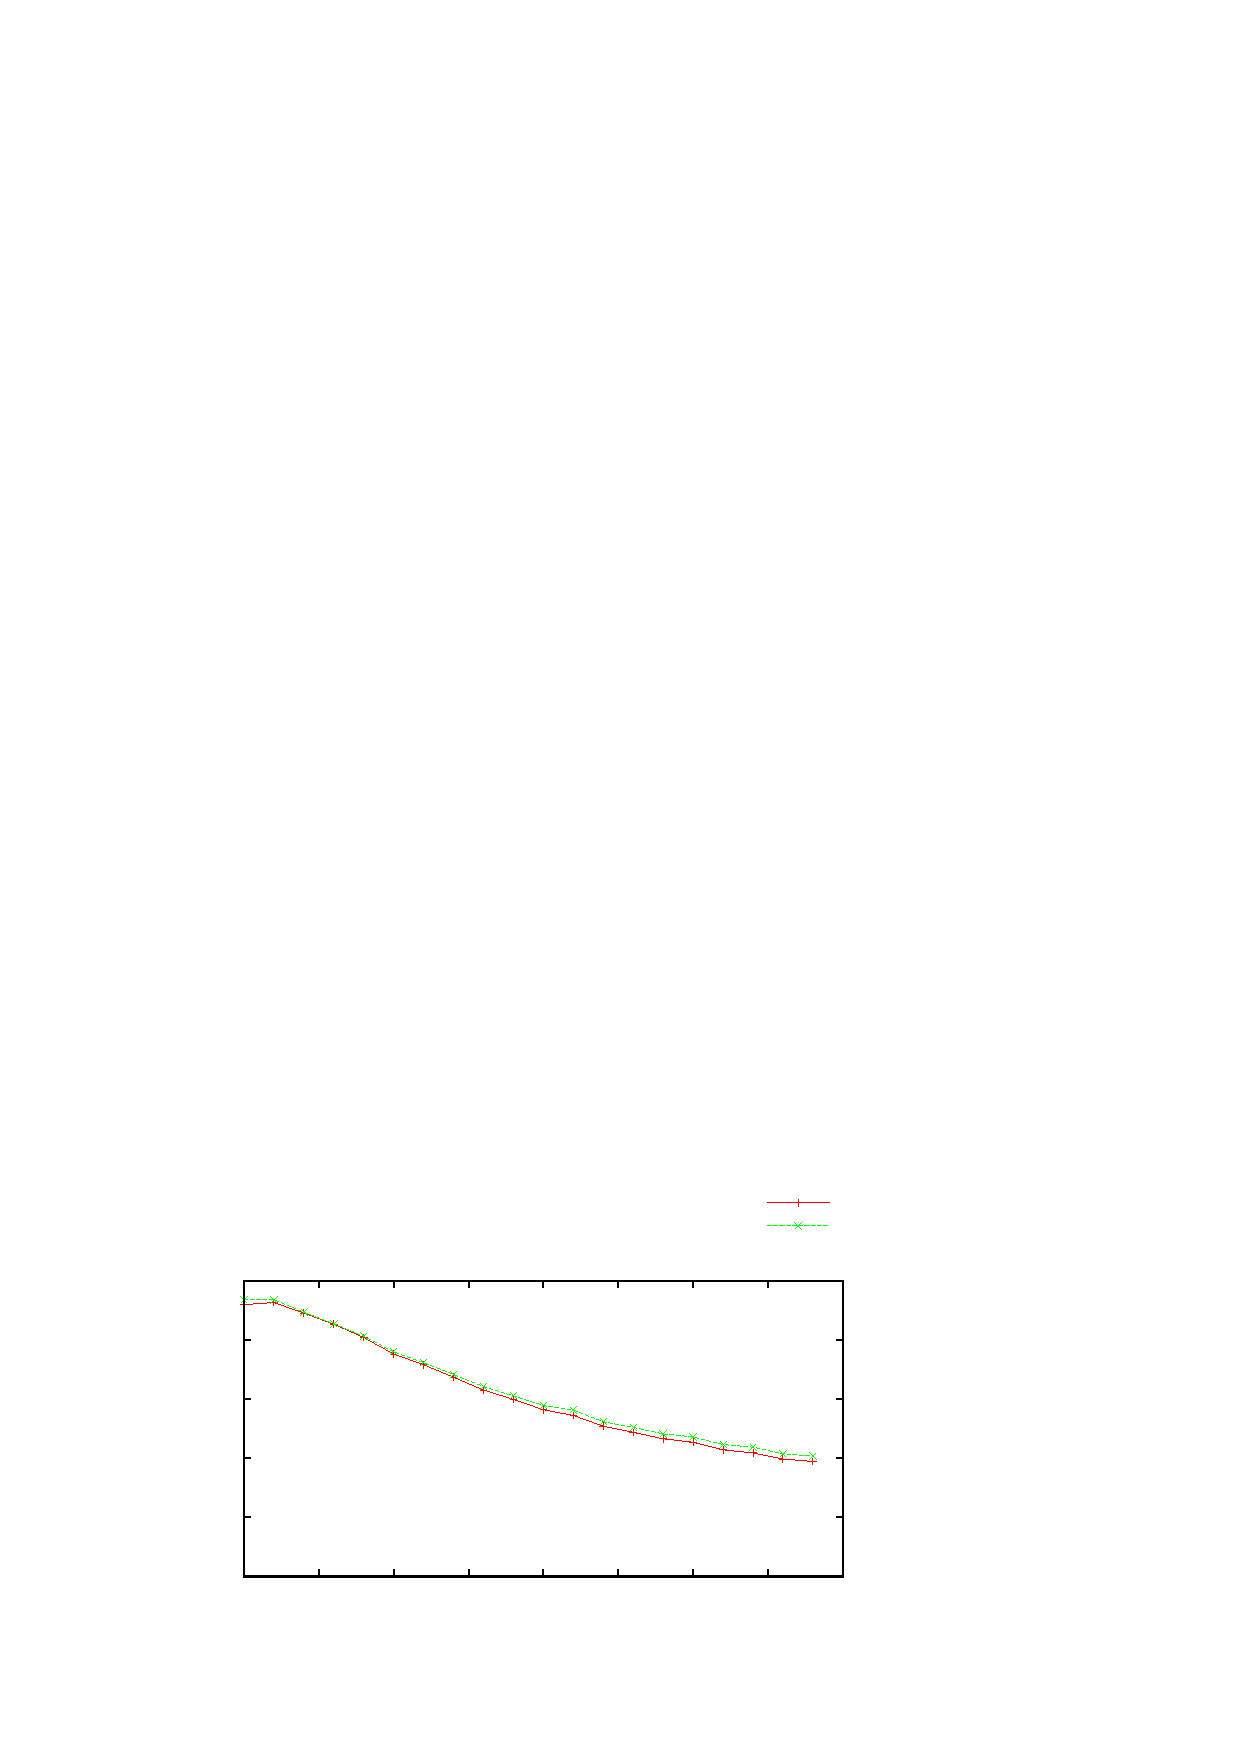
\includegraphics{NaiveVsControlledNodeMemorySkewSelectQuery_BMrate}}%
    \gplfronttext
  \end{picture}%
\endgroup

	\caption{Branch Misprediction Rate}
	\label{fig:NaiveVsControlledNodeMemorySkewSelectQueryBMrate}
\end{subfigure}

\begin{subfigure}{0.48\textwidth}
	% GNUPLOT: LaTeX picture with Postscript
\begingroup
  \makeatletter
  \providecommand\color[2][]{%
    \GenericError{(gnuplot) \space\space\space\@spaces}{%
      Package color not loaded in conjunction with
      terminal option `colourtext'%
    }{See the gnuplot documentation for explanation.%
    }{Either use 'blacktext' in gnuplot or load the package
      color.sty in LaTeX.}%
    \renewcommand\color[2][]{}%
  }%
  \providecommand\includegraphics[2][]{%
    \GenericError{(gnuplot) \space\space\space\@spaces}{%
      Package graphicx or graphics not loaded%
    }{See the gnuplot documentation for explanation.%
    }{The gnuplot epslatex terminal needs graphicx.sty or graphics.sty.}%
    \renewcommand\includegraphics[2][]{}%
  }%
  \providecommand\rotatebox[2]{#2}%
  \@ifundefined{ifGPcolor}{%
    \newif\ifGPcolor
    \GPcolortrue
  }{}%
  \@ifundefined{ifGPblacktext}{%
    \newif\ifGPblacktext
    \GPblacktexttrue
  }{}%
  % define a \g@addto@macro without @ in the name:
  \let\gplgaddtomacro\g@addto@macro
  % define empty templates for all commands taking text:
  \gdef\gplbacktext{}%
  \gdef\gplfronttext{}%
  \makeatother
  \ifGPblacktext
    % no textcolor at all
    \def\colorrgb#1{}%
    \def\colorgray#1{}%
  \else
    % gray or color?
    \ifGPcolor
      \def\colorrgb#1{\color[rgb]{#1}}%
      \def\colorgray#1{\color[gray]{#1}}%
      \expandafter\def\csname LTw\endcsname{\color{white}}%
      \expandafter\def\csname LTb\endcsname{\color{black}}%
      \expandafter\def\csname LTa\endcsname{\color{black}}%
      \expandafter\def\csname LT0\endcsname{\color[rgb]{1,0,0}}%
      \expandafter\def\csname LT1\endcsname{\color[rgb]{0,1,0}}%
      \expandafter\def\csname LT2\endcsname{\color[rgb]{0,0,1}}%
      \expandafter\def\csname LT3\endcsname{\color[rgb]{1,0,1}}%
      \expandafter\def\csname LT4\endcsname{\color[rgb]{0,1,1}}%
      \expandafter\def\csname LT5\endcsname{\color[rgb]{1,1,0}}%
      \expandafter\def\csname LT6\endcsname{\color[rgb]{0,0,0}}%
      \expandafter\def\csname LT7\endcsname{\color[rgb]{1,0.3,0}}%
      \expandafter\def\csname LT8\endcsname{\color[rgb]{0.5,0.5,0.5}}%
    \else
      % gray
      \def\colorrgb#1{\color{black}}%
      \def\colorgray#1{\color[gray]{#1}}%
      \expandafter\def\csname LTw\endcsname{\color{white}}%
      \expandafter\def\csname LTb\endcsname{\color{black}}%
      \expandafter\def\csname LTa\endcsname{\color{black}}%
      \expandafter\def\csname LT0\endcsname{\color{black}}%
      \expandafter\def\csname LT1\endcsname{\color{black}}%
      \expandafter\def\csname LT2\endcsname{\color{black}}%
      \expandafter\def\csname LT3\endcsname{\color{black}}%
      \expandafter\def\csname LT4\endcsname{\color{black}}%
      \expandafter\def\csname LT5\endcsname{\color{black}}%
      \expandafter\def\csname LT6\endcsname{\color{black}}%
      \expandafter\def\csname LT7\endcsname{\color{black}}%
      \expandafter\def\csname LT8\endcsname{\color{black}}%
    \fi
  \fi
  \setlength{\unitlength}{0.0500bp}%
  \begin{picture}(8062.00,4752.00)%
    \gplgaddtomacro\gplbacktext{%
      \csname LTb\endcsname%
      \put(1474,704){\makebox(0,0)[r]{\strut{} 0}}%
      \put(1474,1244){\makebox(0,0)[r]{\strut{} 200000}}%
      \put(1474,1785){\makebox(0,0)[r]{\strut{} 400000}}%
      \put(1474,2325){\makebox(0,0)[r]{\strut{} 600000}}%
      \put(1474,2866){\makebox(0,0)[r]{\strut{} 800000}}%
      \put(1474,3406){\makebox(0,0)[r]{\strut{} 1e+06}}%
      \put(1474,3947){\makebox(0,0)[r]{\strut{} 1.2e+06}}%
      \put(1474,4487){\makebox(0,0)[r]{\strut{} 1.4e+06}}%
      \put(1606,484){\makebox(0,0){\strut{} 2}}%
      \put(2363,484){\makebox(0,0){\strut{} 2.5}}%
      \put(3121,484){\makebox(0,0){\strut{} 3}}%
      \put(3878,484){\makebox(0,0){\strut{} 3.5}}%
      \put(4636,484){\makebox(0,0){\strut{} 4}}%
      \put(5393,484){\makebox(0,0){\strut{} 4.5}}%
      \put(6150,484){\makebox(0,0){\strut{} 5}}%
      \put(6908,484){\makebox(0,0){\strut{} 5.5}}%
      \put(7665,484){\makebox(0,0){\strut{} 6}}%
      \put(176,2595){\rotatebox{-270}{\makebox(0,0){\strut{}Cache Misses}}}%
      \put(4635,154){\makebox(0,0){\strut{}Skew}}%
    }%
    \gplgaddtomacro\gplfronttext{%
      \csname LTb\endcsname%
      \put(6678,1097){\makebox(0,0)[r]{\strut{}Naive L1 $mr\sigma=$0.302}}%
      \csname LTb\endcsname%
      \put(6678,877){\makebox(0,0)[r]{\strut{}ControlledNodeMemory L1 $mr\sigma=$2.589}}%
    }%
    \gplbacktext
    \put(0,0){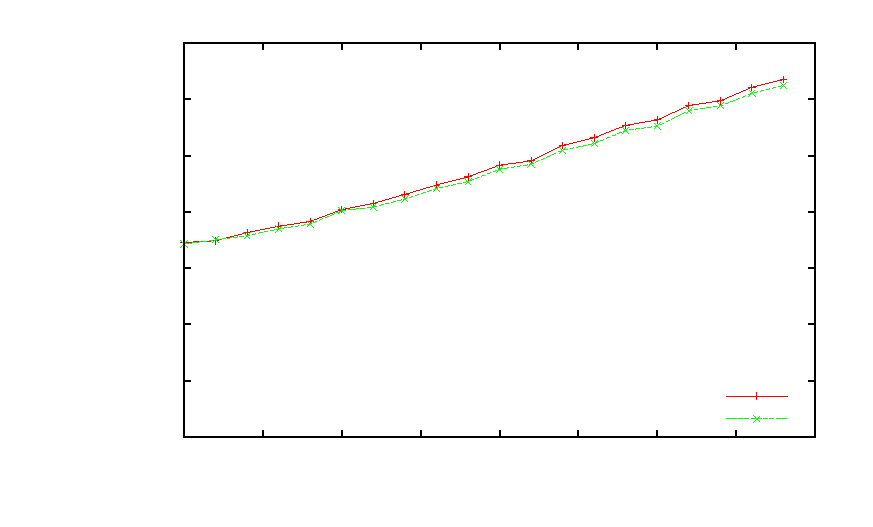
\includegraphics{L1NaiveVsControlledNodeMemorySkewSelectQueryCacheMisses}}%
    \gplfronttext
  \end{picture}%
\endgroup

	\caption{Level 1 Data Cache Misses}
	\label{fig:L1NaiveControlledNodeMemorySelectSkewCacheMisses}
\end{subfigure}
\hfill
\begin{subfigure}{0.48\textwidth}
 	% GNUPLOT: LaTeX picture with Postscript
\begingroup
  \makeatletter
  \providecommand\color[2][]{%
    \GenericError{(gnuplot) \space\space\space\@spaces}{%
      Package color not loaded in conjunction with
      terminal option `colourtext'%
    }{See the gnuplot documentation for explanation.%
    }{Either use 'blacktext' in gnuplot or load the package
      color.sty in LaTeX.}%
    \renewcommand\color[2][]{}%
  }%
  \providecommand\includegraphics[2][]{%
    \GenericError{(gnuplot) \space\space\space\@spaces}{%
      Package graphicx or graphics not loaded%
    }{See the gnuplot documentation for explanation.%
    }{The gnuplot epslatex terminal needs graphicx.sty or graphics.sty.}%
    \renewcommand\includegraphics[2][]{}%
  }%
  \providecommand\rotatebox[2]{#2}%
  \@ifundefined{ifGPcolor}{%
    \newif\ifGPcolor
    \GPcolortrue
  }{}%
  \@ifundefined{ifGPblacktext}{%
    \newif\ifGPblacktext
    \GPblacktexttrue
  }{}%
  % define a \g@addto@macro without @ in the name:
  \let\gplgaddtomacro\g@addto@macro
  % define empty templates for all commands taking text:
  \gdef\gplbacktext{}%
  \gdef\gplfronttext{}%
  \makeatother
  \ifGPblacktext
    % no textcolor at all
    \def\colorrgb#1{}%
    \def\colorgray#1{}%
  \else
    % gray or color?
    \ifGPcolor
      \def\colorrgb#1{\color[rgb]{#1}}%
      \def\colorgray#1{\color[gray]{#1}}%
      \expandafter\def\csname LTw\endcsname{\color{white}}%
      \expandafter\def\csname LTb\endcsname{\color{black}}%
      \expandafter\def\csname LTa\endcsname{\color{black}}%
      \expandafter\def\csname LT0\endcsname{\color[rgb]{1,0,0}}%
      \expandafter\def\csname LT1\endcsname{\color[rgb]{0,1,0}}%
      \expandafter\def\csname LT2\endcsname{\color[rgb]{0,0,1}}%
      \expandafter\def\csname LT3\endcsname{\color[rgb]{1,0,1}}%
      \expandafter\def\csname LT4\endcsname{\color[rgb]{0,1,1}}%
      \expandafter\def\csname LT5\endcsname{\color[rgb]{1,1,0}}%
      \expandafter\def\csname LT6\endcsname{\color[rgb]{0,0,0}}%
      \expandafter\def\csname LT7\endcsname{\color[rgb]{1,0.3,0}}%
      \expandafter\def\csname LT8\endcsname{\color[rgb]{0.5,0.5,0.5}}%
    \else
      % gray
      \def\colorrgb#1{\color{black}}%
      \def\colorgray#1{\color[gray]{#1}}%
      \expandafter\def\csname LTw\endcsname{\color{white}}%
      \expandafter\def\csname LTb\endcsname{\color{black}}%
      \expandafter\def\csname LTa\endcsname{\color{black}}%
      \expandafter\def\csname LT0\endcsname{\color{black}}%
      \expandafter\def\csname LT1\endcsname{\color{black}}%
      \expandafter\def\csname LT2\endcsname{\color{black}}%
      \expandafter\def\csname LT3\endcsname{\color{black}}%
      \expandafter\def\csname LT4\endcsname{\color{black}}%
      \expandafter\def\csname LT5\endcsname{\color{black}}%
      \expandafter\def\csname LT6\endcsname{\color{black}}%
      \expandafter\def\csname LT7\endcsname{\color{black}}%
      \expandafter\def\csname LT8\endcsname{\color{black}}%
    \fi
  \fi
  \setlength{\unitlength}{0.0500bp}%
  \begin{picture}(4608.00,3600.00)%
    \gplgaddtomacro\gplbacktext{%
      \csname LTb\endcsname%
      \put(804,384){\makebox(0,0)[r]{\strut{} 0}}%
      \put(804,768){\makebox(0,0)[r]{\strut{} 2e+06}}%
      \put(804,1152){\makebox(0,0)[r]{\strut{} 4e+06}}%
      \put(804,1536){\makebox(0,0)[r]{\strut{} 6e+06}}%
      \put(804,1920){\makebox(0,0)[r]{\strut{} 8e+06}}%
      \put(804,2303){\makebox(0,0)[r]{\strut{} 1e+07}}%
      \put(804,2687){\makebox(0,0)[r]{\strut{} 1.2e+07}}%
      \put(804,3071){\makebox(0,0)[r]{\strut{} 1.4e+07}}%
      \put(804,3455){\makebox(0,0)[r]{\strut{} 1.6e+07}}%
      \put(876,264){\makebox(0,0){\strut{} 2}}%
      \put(1315,264){\makebox(0,0){\strut{} 2.5}}%
      \put(1755,264){\makebox(0,0){\strut{} 3}}%
      \put(2194,264){\makebox(0,0){\strut{} 3.5}}%
      \put(2634,264){\makebox(0,0){\strut{} 4}}%
      \put(3073,264){\makebox(0,0){\strut{} 4.5}}%
      \put(3512,264){\makebox(0,0){\strut{} 5}}%
      \put(3952,264){\makebox(0,0){\strut{} 5.5}}%
      \put(4391,264){\makebox(0,0){\strut{} 6}}%
      \put(96,1919){\rotatebox{-270}{\makebox(0,0){\strut{}Cache Misses}}}%
      \put(2633,84){\makebox(0,0){\strut{}Skew}}%
    }%
    \gplgaddtomacro\gplfronttext{%
      \csname LTb\endcsname%
      \put(1673,3332){\makebox(0,0)[r]{\strut{}Naive L2}}%
      \csname LTb\endcsname%
      \put(1673,3212){\makebox(0,0)[r]{\strut{}Naive L3}}%
      \csname LTb\endcsname%
      \put(3824,3332){\makebox(0,0)[r]{\strut{}ControlledNodeMemory L2}}%
      \csname LTb\endcsname%
      \put(3824,3212){\makebox(0,0)[r]{\strut{}ControlledNodeMemory L3}}%
    }%
    \gplbacktext
    \put(0,0){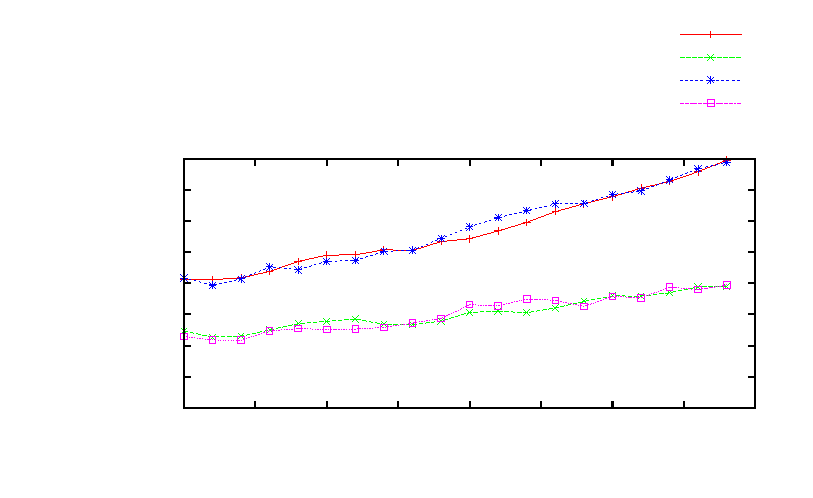
\includegraphics{L2L3NaiveVsControlledNodeMemorySkewSelectQueryCacheMisses}}%
    \gplfronttext
  \end{picture}%
\endgroup

	\caption{Level 2 Data and 3 Total Cache Misses}
	\label{fig:L2L3NaiveControlledNodeMemorySelectSkewCacheMisses}
\end{subfigure}

\begin{subfigure}{0.48\textwidth}
	% GNUPLOT: LaTeX picture with Postscript
\begingroup
  \makeatletter
  \providecommand\color[2][]{%
    \GenericError{(gnuplot) \space\space\space\@spaces}{%
      Package color not loaded in conjunction with
      terminal option `colourtext'%
    }{See the gnuplot documentation for explanation.%
    }{Either use 'blacktext' in gnuplot or load the package
      color.sty in LaTeX.}%
    \renewcommand\color[2][]{}%
  }%
  \providecommand\includegraphics[2][]{%
    \GenericError{(gnuplot) \space\space\space\@spaces}{%
      Package graphicx or graphics not loaded%
    }{See the gnuplot documentation for explanation.%
    }{The gnuplot epslatex terminal needs graphicx.sty or graphics.sty.}%
    \renewcommand\includegraphics[2][]{}%
  }%
  \providecommand\rotatebox[2]{#2}%
  \@ifundefined{ifGPcolor}{%
    \newif\ifGPcolor
    \GPcolortrue
  }{}%
  \@ifundefined{ifGPblacktext}{%
    \newif\ifGPblacktext
    \GPblacktexttrue
  }{}%
  % define a \g@addto@macro without @ in the name:
  \let\gplgaddtomacro\g@addto@macro
  % define empty templates for all commands taking text:
  \gdef\gplbacktext{}%
  \gdef\gplfronttext{}%
  \makeatother
  \ifGPblacktext
    % no textcolor at all
    \def\colorrgb#1{}%
    \def\colorgray#1{}%
  \else
    % gray or color?
    \ifGPcolor
      \def\colorrgb#1{\color[rgb]{#1}}%
      \def\colorgray#1{\color[gray]{#1}}%
      \expandafter\def\csname LTw\endcsname{\color{white}}%
      \expandafter\def\csname LTb\endcsname{\color{black}}%
      \expandafter\def\csname LTa\endcsname{\color{black}}%
      \expandafter\def\csname LT0\endcsname{\color[rgb]{1,0,0}}%
      \expandafter\def\csname LT1\endcsname{\color[rgb]{0,1,0}}%
      \expandafter\def\csname LT2\endcsname{\color[rgb]{0,0,1}}%
      \expandafter\def\csname LT3\endcsname{\color[rgb]{1,0,1}}%
      \expandafter\def\csname LT4\endcsname{\color[rgb]{0,1,1}}%
      \expandafter\def\csname LT5\endcsname{\color[rgb]{1,1,0}}%
      \expandafter\def\csname LT6\endcsname{\color[rgb]{0,0,0}}%
      \expandafter\def\csname LT7\endcsname{\color[rgb]{1,0.3,0}}%
      \expandafter\def\csname LT8\endcsname{\color[rgb]{0.5,0.5,0.5}}%
    \else
      % gray
      \def\colorrgb#1{\color{black}}%
      \def\colorgray#1{\color[gray]{#1}}%
      \expandafter\def\csname LTw\endcsname{\color{white}}%
      \expandafter\def\csname LTb\endcsname{\color{black}}%
      \expandafter\def\csname LTa\endcsname{\color{black}}%
      \expandafter\def\csname LT0\endcsname{\color{black}}%
      \expandafter\def\csname LT1\endcsname{\color{black}}%
      \expandafter\def\csname LT2\endcsname{\color{black}}%
      \expandafter\def\csname LT3\endcsname{\color{black}}%
      \expandafter\def\csname LT4\endcsname{\color{black}}%
      \expandafter\def\csname LT5\endcsname{\color{black}}%
      \expandafter\def\csname LT6\endcsname{\color{black}}%
      \expandafter\def\csname LT7\endcsname{\color{black}}%
      \expandafter\def\csname LT8\endcsname{\color{black}}%
    \fi
  \fi
  \setlength{\unitlength}{0.0500bp}%
  \begin{picture}(7488.00,4752.00)%
    \gplgaddtomacro\gplbacktext{%
      \csname LTb\endcsname%
      \put(1474,704){\makebox(0,0)[r]{\strut{} 0}}%
      \put(1474,1150){\makebox(0,0)[r]{\strut{} 200000}}%
      \put(1474,1596){\makebox(0,0)[r]{\strut{} 400000}}%
      \put(1474,2042){\makebox(0,0)[r]{\strut{} 600000}}%
      \put(1474,2489){\makebox(0,0)[r]{\strut{} 800000}}%
      \put(1474,2935){\makebox(0,0)[r]{\strut{} 1e+06}}%
      \put(1474,3381){\makebox(0,0)[r]{\strut{} 1.2e+06}}%
      \put(1474,3827){\makebox(0,0)[r]{\strut{} 1.4e+06}}%
      \put(1606,484){\makebox(0,0){\strut{} 2}}%
      \put(2292,484){\makebox(0,0){\strut{} 2.5}}%
      \put(2977,484){\makebox(0,0){\strut{} 3}}%
      \put(3663,484){\makebox(0,0){\strut{} 3.5}}%
      \put(4349,484){\makebox(0,0){\strut{} 4}}%
      \put(5034,484){\makebox(0,0){\strut{} 4.5}}%
      \put(5720,484){\makebox(0,0){\strut{} 5}}%
      \put(6405,484){\makebox(0,0){\strut{} 5.5}}%
      \put(7091,484){\makebox(0,0){\strut{} 6}}%
      \put(176,2265){\rotatebox{-270}{\makebox(0,0){\strut{}L2 Cache miss rate}}}%
      \put(4348,154){\makebox(0,0){\strut{}Skew}}%
    }%
    \gplgaddtomacro\gplfronttext{%
      \csname LTb\endcsname%
      \put(6236,4579){\makebox(0,0)[r]{\strut{}Naive $mr\hat{\sigma}=$4.438 $avg\hat{\sigma}=$1.58}}%
      \csname LTb\endcsname%
      \put(6236,4359){\makebox(0,0)[r]{\strut{}ControlledNodeMemory $mr\hat{\sigma}=$27.269 $avg\hat{\sigma}=$6.47}}%
    }%
    \gplbacktext
    \put(0,0){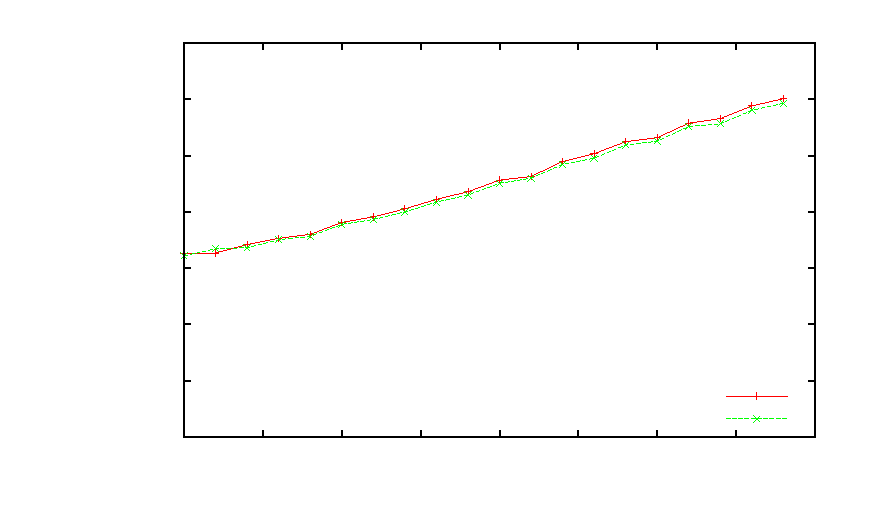
\includegraphics{NaiveVsControlledNodeMemorySkewSelectQuery_L2_DCMrate}}%
    \gplfronttext
  \end{picture}%
\endgroup

	\caption{Level 2 Data Cache Miss Rate}
	\label{fig:NaiveVsControlledNodeMemorySkewSelectQuery_L2_DCMrate}
\end{subfigure}
\hfill
\begin{subfigure}{0.48\textwidth}
	% GNUPLOT: LaTeX picture with Postscript
\begingroup
  \makeatletter
  \providecommand\color[2][]{%
    \GenericError{(gnuplot) \space\space\space\@spaces}{%
      Package color not loaded in conjunction with
      terminal option `colourtext'%
    }{See the gnuplot documentation for explanation.%
    }{Either use 'blacktext' in gnuplot or load the package
      color.sty in LaTeX.}%
    \renewcommand\color[2][]{}%
  }%
  \providecommand\includegraphics[2][]{%
    \GenericError{(gnuplot) \space\space\space\@spaces}{%
      Package graphicx or graphics not loaded%
    }{See the gnuplot documentation for explanation.%
    }{The gnuplot epslatex terminal needs graphicx.sty or graphics.sty.}%
    \renewcommand\includegraphics[2][]{}%
  }%
  \providecommand\rotatebox[2]{#2}%
  \@ifundefined{ifGPcolor}{%
    \newif\ifGPcolor
    \GPcolortrue
  }{}%
  \@ifundefined{ifGPblacktext}{%
    \newif\ifGPblacktext
    \GPblacktexttrue
  }{}%
  % define a \g@addto@macro without @ in the name:
  \let\gplgaddtomacro\g@addto@macro
  % define empty templates for all commands taking text:
  \gdef\gplbacktext{}%
  \gdef\gplfronttext{}%
  \makeatother
  \ifGPblacktext
    % no textcolor at all
    \def\colorrgb#1{}%
    \def\colorgray#1{}%
  \else
    % gray or color?
    \ifGPcolor
      \def\colorrgb#1{\color[rgb]{#1}}%
      \def\colorgray#1{\color[gray]{#1}}%
      \expandafter\def\csname LTw\endcsname{\color{white}}%
      \expandafter\def\csname LTb\endcsname{\color{black}}%
      \expandafter\def\csname LTa\endcsname{\color{black}}%
      \expandafter\def\csname LT0\endcsname{\color[rgb]{1,0,0}}%
      \expandafter\def\csname LT1\endcsname{\color[rgb]{0,1,0}}%
      \expandafter\def\csname LT2\endcsname{\color[rgb]{0,0,1}}%
      \expandafter\def\csname LT3\endcsname{\color[rgb]{1,0,1}}%
      \expandafter\def\csname LT4\endcsname{\color[rgb]{0,1,1}}%
      \expandafter\def\csname LT5\endcsname{\color[rgb]{1,1,0}}%
      \expandafter\def\csname LT6\endcsname{\color[rgb]{0,0,0}}%
      \expandafter\def\csname LT7\endcsname{\color[rgb]{1,0.3,0}}%
      \expandafter\def\csname LT8\endcsname{\color[rgb]{0.5,0.5,0.5}}%
    \else
      % gray
      \def\colorrgb#1{\color{black}}%
      \def\colorgray#1{\color[gray]{#1}}%
      \expandafter\def\csname LTw\endcsname{\color{white}}%
      \expandafter\def\csname LTb\endcsname{\color{black}}%
      \expandafter\def\csname LTa\endcsname{\color{black}}%
      \expandafter\def\csname LT0\endcsname{\color{black}}%
      \expandafter\def\csname LT1\endcsname{\color{black}}%
      \expandafter\def\csname LT2\endcsname{\color{black}}%
      \expandafter\def\csname LT3\endcsname{\color{black}}%
      \expandafter\def\csname LT4\endcsname{\color{black}}%
      \expandafter\def\csname LT5\endcsname{\color{black}}%
      \expandafter\def\csname LT6\endcsname{\color{black}}%
      \expandafter\def\csname LT7\endcsname{\color{black}}%
      \expandafter\def\csname LT8\endcsname{\color{black}}%
    \fi
  \fi
  \setlength{\unitlength}{0.0500bp}%
  \begin{picture}(4608.00,3600.00)%
    \gplgaddtomacro\gplbacktext{%
      \csname LTb\endcsname%
      \put(804,384){\makebox(0,0)[r]{\strut{} 0}}%
      \put(804,823){\makebox(0,0)[r]{\strut{} 200000}}%
      \put(804,1261){\makebox(0,0)[r]{\strut{} 400000}}%
      \put(804,1700){\makebox(0,0)[r]{\strut{} 600000}}%
      \put(804,2139){\makebox(0,0)[r]{\strut{} 800000}}%
      \put(804,2578){\makebox(0,0)[r]{\strut{} 1e+06}}%
      \put(804,3016){\makebox(0,0)[r]{\strut{} 1.2e+06}}%
      \put(804,3455){\makebox(0,0)[r]{\strut{} 1.4e+06}}%
      \put(876,264){\makebox(0,0){\strut{} 2}}%
      \put(1315,264){\makebox(0,0){\strut{} 2.5}}%
      \put(1755,264){\makebox(0,0){\strut{} 3}}%
      \put(2194,264){\makebox(0,0){\strut{} 3.5}}%
      \put(2634,264){\makebox(0,0){\strut{} 4}}%
      \put(3073,264){\makebox(0,0){\strut{} 4.5}}%
      \put(3512,264){\makebox(0,0){\strut{} 5}}%
      \put(3952,264){\makebox(0,0){\strut{} 5.5}}%
      \put(4391,264){\makebox(0,0){\strut{} 6}}%
      \put(96,1919){\rotatebox{-270}{\makebox(0,0){\strut{}TLB}}}%
      \put(2633,84){\makebox(0,0){\strut{}Skew}}%
    }%
    \gplgaddtomacro\gplfronttext{%
      \csname LTb\endcsname%
      \put(3824,3332){\makebox(0,0)[r]{\strut{}NaiveInteger}}%
      \csname LTb\endcsname%
      \put(3824,3212){\makebox(0,0)[r]{\strut{}ControlledMemory}}%
    }%
    \gplbacktext
    \put(0,0){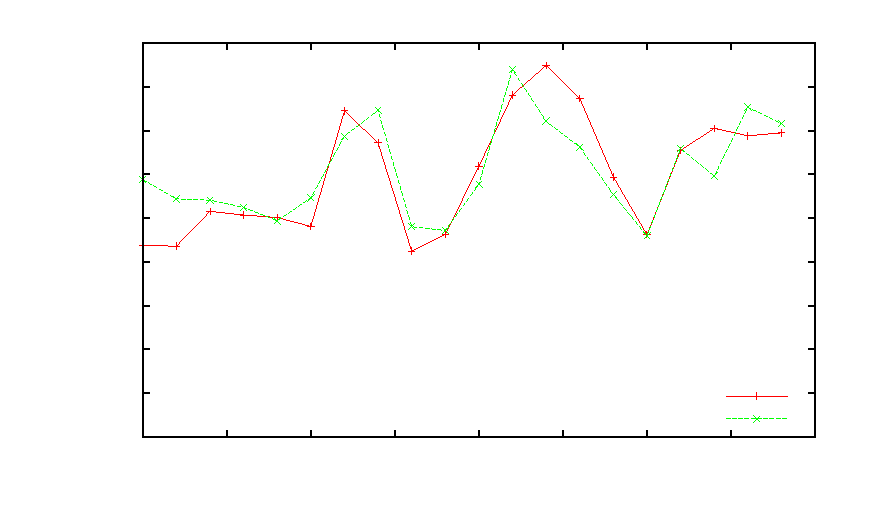
\includegraphics{NaiveVsControlledNodeMemorySkewSelectQueryTLB}}%
    \gplfronttext
  \end{picture}%
\endgroup

	\caption{TLB Misses}
	\label{fig:NaiveVsControlledNodeMemorySkewSelectQueryTLB}
\end{subfigure}

\caption{Various measurements for Select queries on NaiveInteger and ControlledNodeMemory wavelet trees with various skew.}
\label{fig:NaiveVsControlledNodeMemorySkewSelectQuery}

\end{figure}


\restoregeometry



\paragraph{Why skewing is not an improvement}~\\
When we skew the tree we do not split the alphabet into equal sizes and therefore add more data to the right side of the tree than to the left. 
This increases the hight of the tree and we need to look at more nodes to find the result than if the tree was balanced and as a result of this we do more work because we have to access more nodes and bitmaps.

We had hoped to reduce the amount of branch mispredictions and cache misses enough that they would reduce the running time more than the increase from having a deeper tree structure.
Sadly, this was not the case. We believe the reason it worked so well for Brodal et. al.\cite{gerthSkewedBinarySearchTrees} but not for us, is that the binary search trees they worked on have much less work involved in traversing each node and so most of the time is spent traversing from node to node.
In rank and select queries on a wavelet tree, most of the time is spent calculating the binary ranks of the bitmaps of each node as well as other calculations performed for each node.

Skewing the tree can help reduce the time spent between nodes by reducing the performance hits from branch mispredictions and cache misses that arise because of the unpredictable nature of a balanced tree traversal, by making the path of the traversal much more predictable and pre-loadable.
It can not, however, help reduce the work performed when reaching each node, and when the total time spent on that work is proportional to the height of the tree, as it is with a wavelet tree, it is a great reduction in speed to skew the tree and thereby increase the height of the tree.
The total intra-node work is proportional to the height of the tree because that work is proportional to the bitmap size and the bitmap sizes are inversely proportional to the number of nodes in the same layer, as the size of all the bitmaps in one layer sum up to $n$. A skewed tree does not have each layer filled with nodes and so the rest of the bitmaps on those levels become larger, as well as any extra layer produced by skewing the tree means another number of bitmaps must appear with combined size $n$.


